%%% EHS submission version (Cambridge cup-journal class). Compile with pdflatex + biber.
%%% cup-journal.cls + cup-logo-new.pdf must be present (from the Cambridge Medium template).
%%% EHS article type: Original Research Article (select this category in ScholarOne).
%%%   The cup-journal class only accepts manuscript=article|communication|suppinfo,
%%%   so the printed type banner reads "Article".
%%% Double-blind review: \blindtrue (below) hides the author, affiliation, and the
%%%   identifying data/preregistration links. Set \blindfalse for the camera-ready.
%%% Social media summary (enter in submission portal, <=120 chars):
%%%   NFL coaching lineages inherit a mentor's system, not his success: what
%%%   transmits is largely not what wins.
\documentclass[
  journal=ehs,
  manuscript=article,
  year=2026,
  volume=8,
]{cup-journal}

\usepackage{amsmath}
\usepackage[nopatch]{microtype}
\usepackage{booktabs}
\usepackage{graphicx}

\newif\ifblind
\blindtrue   % double-blind review; set \blindfalse for the de-anonymised camera-ready

\title{Heritability and selection of strategic traits in the NFL coaching tree}

\ifblind
  \author{Anonymised for review}
  \affiliation{Affiliation removed for anonymous review}
\else
  \author{Jon Williamson}
  \affiliation{Williamson Consulting Group, USA}
  \email[Jon Williamson]{jonwilliamson@live.com}
\fi

\addbibresource{refs.bib}

\keywords{cultural evolution, social learning, vertical transmission, heritability, cultural fitness, sport}

\begin{document}

\begin{abstract}
Human expertise is transmitted socially, and where learners have
identifiable teachers it descends a traceable lineage. Cultural-evolution research
has shown how successful sport tactics spread sideways among contemporaries; we ask
instead what descends the mentor-protege lineage. We treat the National Football
League coaching tree as a cultural pedigree and, for a preregistered set of ten
standardized play-calling traits, estimate each trait's transmissibility ($h^{2}$,
mentor-to-protege resemblance from a Bayesian parent-offspring model with a
measurement-error correction) and its selection ($S$, its association with the
coach's wins above replacement, WAR, a roster- and schedule-adjusted estimate of a
coach's own contribution). The ten traits, defined from coaches' play-calling and
in-game decisions, are each a genuine, repeatable individual characteristic
(repeatabilities 0.34 to 0.58), yet transmissibility and selection come apart.
Schematic-identity traits transmit but do not win: shotgun $h^{2}=0.45$ (95\% HDI
$[0.27,0.65]$) with $S=0.08$, and tempo similarly. Offensive aggression is the mirror
image, repeatable ($0.40$) and selected ($S=0.18$, $[0.08,0.27]$) yet not transmitted
($h^{2}=-0.15$); a preregistered contrast confirms it is repeatable but not heritable
($0.55$, $[0.24,0.87]$). Defensive aggression alone both transmits ($h^{2}=0.49$) and
wins ($S=0.15$). We did not observe the predicted negative heritability-fitness
relationship (Spearman $+0.32$, $[-0.54,0.69]$); with few transitions and wide
intervals this is inconclusive, and transmission and selection appear largely
decoupled rather than traded off. Coaching lineages propagate a mentor's system, not
his success: a protege inherits how his teams will play, not the behavior that wins,
which spreads sideways among contemporaries rather than down the tree.
\end{abstract}

\section{Introduction}
%% ----------------------------------------------------------------------------

Human skilled practice is transmitted socially, and where practitioners learn from
identifiable teachers the transmission runs along a traceable lineage. Coaching in
the National Football League (NFL) is a case where that lineage is unusually legible
by the standards of human apprenticeship. Head coaches hire assistants, assistants
become coordinators, coordinators are promoted to head coach, and the record of who
worked under whom is documented season by season. The result is a ``coaching tree'':
a directed network of mentor--protege ties along which styles of play, and coaching
ability itself, are widely believed to descend. Popular accounts speak of the Walsh
tree or the Belichick tree much as a breeder speaks of a bloodline, and teams often
hire on that pedigree logic, in the belief that working under a successful coach
transfers winning approaches and strategic expertise.

Cultural evolution treats socially learned behavior as a second inheritance system,
one that, like the genetic system, is transmitted, varies, and is subject to
selection \parencite{cavallisforza1981, boydricherson1985, henrich2016}. Much of the
human capital that distinguishes experts, from surgeons to craftspeople to coaches,
is acquired by working under a more accomplished practitioner rather than from
books, so expertise descends along chains of apprenticeship \parencite{henrich2016}.
Measuring vertical transmission in such chains is nonetheless hard: it requires
observing the same behavior in both teacher and learner, on a comparable scale, with
the lineage known, and such behavioral lineages are seldom that legible in humans.
Professional sport is an exception, because the record of who coached under whom is
public and the behavior itself is recorded play by play.

Recent work has begun to treat sport tactics as a cultural-evolutionary system.
\textcite{mesoudi2020}, in this journal, analyzed the cultural evolution of
association-football (soccer) formations across more than nine thousand matches in
five European leagues and showed that a manager's use of the era's dominant formation
(the 4-2-3-1) tracked both his own recent use of and success with it and how widely it
was used across contemporary managers. Formation choice was guided by strategic social
learning, and a successful tactic diffused as managers copied it from their peers: a
horizontal channel, transmission among contemporaries. That study measured the
horizontal channel and named two things it could not reach as open questions:
transmission down mentor--protege lineages (i.e., the vertical channel) and the flow
of influence along the social-network ties that connect managers, for which the author
offered the lineage of managers who carry Marcelo Bielsa's approach as the motivating
example. The present paper takes up those questions in the NFL. Cultural transmission
theory distinguishes vertical transmission, from a parent-like model to a learner,
from horizontal transmission among contemporaries, and the two need not carry the same
traits \parencite{cavallisforza1981, boydricherson1985}. As we will show, the vertical
and horizontal channels in coaching move different strategic traits, so the two
studies are complementary halves of one picture.

To ask how faithfully behavior descends such a lineage, we borrow the toolkit
quantitative genetics built for that decomposition. Two quantities anchor it.
Repeatability is the share of a trait's variance that is a stable property of the
individual rather than occasion-to-occasion noise, and it sets an upper bound on how
much of the trait can be transmitted at all. Heritability is the share actually
passed to descendants; in a parent-offspring design it is read directly from the
resemblance between parent and offspring phenotypes, with no need for an assumed
relatedness matrix \parencite{falconermackay1996}. The same variance-partitioning logic
extends from classical pedigrees to repeated measures through the mixed-model animal
model \parencite{wilson2010, nakagawa2010}, and dual-inheritance theory has long held
that it applies to culturally transmitted traits as well as genetic ones
\parencite{cavallisforza1981}. Such systems, in which both the lineage and the
phenotype are observed directly rather than inferred, are uncommon for culture; the
coaching tree is one.

We use these tools to place each trait on two axes. The first is transmissibility,
the cultural analog of heritability $h^{2}$: how strongly a protege's own
head-coaching style resembles the style of the coach they apprenticed under. The
second is selection $S$: how strongly a trait covaries with a coach's success,
measured by wins above replacement (WAR), an estimate designed to adjust for roster
and schedule and isolate the coaching contribution. In biological
populations the two are famously in tension. Fisher's fundamental theorem implies
that selection consumes the additive genetic variance of the traits most closely
tied to fitness, so those traits should be the \emph{least} heritable
\parencite{fisher1930}. The prediction holds across taxa: \textcite{mousseauroff1987}
found life-history traits, those nearest fitness, markedly less heritable than
morphological ones, and \textcite{kruuk2000} report a rank correlation near $-0.8$
between the heritability of a suite of red-deer traits and their association with
fitness. Whether an analogous tension arises in a cultural system, where
inheritance is social learning rather than meiosis and the variance-depleting logic
of Fisher's theorem need not apply, is unknown.

We proceed in three steps. First, we ask whether these play-calling tendencies are
genuine, stable properties of a coach at all rather than artifacts of a roster or a
season. Second, we ask whether they transmit from mentor to protege down the lineage
(the heritability $h^{2}$). Third, we ask whether they predict a coach's success (the
selection $S$). The question that ties the three together is whether the traits that
transmit are the same traits that win. We separate strategy into two
families. \emph{Approach-to-scenarios} traits describe how aggressively a coach
attacks game situations (going for it on fourth down, passing in neutral
situations, throwing beyond the first-down marker, attempting two-point
conversions, and on defense loading the box, sending extra rushers, and playing man
coverage). \emph{Schematic-identity} traits describe the formational signature of a
team (how much it operates from shotgun, and how fast it plays). The split is
cleanest on offense; as we discuss below, defensive ``aggression'' mixes an
attitudinal and a schematic component. Our preregistered hypotheses were:
\begin{itemize}
  \item[H1.] Approach traits are more strongly selected (predict WAR), while
  identity traits are more strongly inherited (transmit down the tree).
  \item[H2.] Offensive aggression is a repeatable individual trait that is
  nonetheless not heritable: its within-coach repeatability clearly exceeds its
  transmissibility.
  \item[H3.] Across the ten sub-traits, heritability and selection are negatively
  related: the traits that transmit most strongly are not the ones that predict
  winning.
\end{itemize}
These predictions were registered before any confirmatory quantity was computed on
the final measurement pipeline (Section~\ref{sec:methods}).

%% ----------------------------------------------------------------------------
\section{Methods}\label{sec:methods}
%% ----------------------------------------------------------------------------

\subsection{Coaching phenotypes (``genes'')}
We construct standardized coach-season phenotypes from play-by-play data for the
2006--2024 NFL seasons (obtained through \texttt{nfl\_data\_py}; more than 600{,}000
plays). For each of the ten decisions in Table~\ref{tab:traits} we train a
play-level expectation model (gradient-boosted trees) on pre-play game context only,
deliberately excluding season, week, and coach identity, so the baseline reflects
what an average coach would do in identical circumstances and is time-invariant. A
coach-season phenotype is the average deviation of observed behavior from this
expectation. Writing $a_{cj}$ for coach $c$'s action on play $j$ of that coach's
$n_c$ plays in a season (an indicator for the discrete decisions, a continuous value
for pace and the box and rusher counts) and $\hat{a}_{cj}$ for the model's
expectation given that play's pre-snap context, the raw gene is
\begin{equation}
  g_c \;=\; \frac{1}{n_c}\sum_{j=1}^{n_c} a_{cj}
          \;-\; \frac{1}{n_c}\sum_{j=1}^{n_c} \hat{a}_{cj},
  \label{eq:gene}
\end{equation}
and the phenotype is its standardization across coach-seasons,
$\tilde{g}_c = (g_c - \bar{g})/\mathrm{sd}(g)$, where $\bar{g}$ and $\mathrm{sd}(g)$
are the sample mean and standard deviation of $g$ over all coach-seasons; positive
values denote more
aggressive, faster, or more shotgun-oriented play than context predicts. This
residual construction isolates a strategic tendency from forced circumstance: a
coach who goes for it often only because he is always trailing is not thereby
aggressive.

The ten sub-traits are the residuals of ten play-level models (Table~\ref{tab:traits}):
four offensive-aggression decisions (going for it on fourth down, passing versus
running in neutral situations, throwing a pass beyond versus short of the first-down
marker, and attempting a two-point conversion), two tempo behaviors (no-huddle use
and seconds between snaps), three defensive behaviors (defenders in the box, number
of pass rushers, and man versus zone coverage), and shotgun formation use. Each is a
gradient-boosted model on pre-play context (down, distance, field position, score,
clock, and environment), a classifier for the discrete decisions and a regressor for
the continuous ones (pace, box count, rushers). Situational context explains most of
the variance in each decision, leaving the smaller, coach-specific residual we read
as tendency; each model's type and out-of-sample performance are given in
Table~\ref{tab:traits}. The pass-rush count is a partial exception: teams rush four
defenders on the large majority of dropbacks, so pre-play context explains little of
its narrow variance ($R^2$ near 0.05). Because the gene is a mean deviation rather
than an explained-variance quantity, a low $R^2$ here still yields a valid measure of
whether a defense systematically sends more or fewer rushers than expected; the model
supplies an unbiased expectation to residualize against, and the residual retains a
repeatable, transmissible coach signal (Table~\ref{tab:main}). The expectation
models, the leakage controls that keep a
coach's own tendencies out of the yardstick that measures them, and the reliability
weighting are detailed in the next two subsections.

Every play is attributed to the head coach who led the team for that game, so a
within-season head-coaching change splits the season between the two coaches at the
game of the change. Coordinators are not assigned their own phenotype; the
phenotype is defined only at the head-coach level, so a play is attributed to one
coach and never to both a head coach and a coordinator at once. To keep a coach's
own tendencies out of the yardstick that measures them, expectation models are fit
with the scoring coach held out and with cross-fitting folds balanced across eras,
so each play is scored by a model that never trained on that coach.

Ten sub-traits are frozen for the primary analysis (Table~\ref{tab:traits}),
grouped into four gene-level composites (offensive aggression, tempo, defensive
aggression, and shotgun) that serve as labeled exemplars but are not counted as
independent points in the cross-trait test.

\begin{table}[t]
\centering
\caption{The ten frozen sub-traits: gene-level composite, the play-level
expectation model whose residual defines the phenotype and its out-of-sample
performance (AUC for classifiers, $R^2$ for regressors, under grouped resampling
that holds out whole team-years), and the data window. All transitions tested are
offensive-coordinator-to-head-coach except the three defensive traits, which are
defensive-coordinator-to-head-coach.}
\label{tab:traits}
\begin{tabular}{lllll}
\toprule
Sub-trait & Composite & Model & Performance & Window \\
\midrule
Fourth-down  & Offensive aggression & classifier & AUC 0.97 & 2006--2024 \\
Pass-heavy   & Offensive aggression & classifier & AUC 0.78 & 2006--2024 \\
Deep-pass    & Offensive aggression & classifier & AUC 0.73 & 2006--2024 \\
Two-point    & Offensive aggression & classifier & AUC 0.93 & 2006--2024 \\
No-huddle    & Tempo                & classifier & AUC 0.77 & 2006--2024 \\
Pace         & Tempo                & regressor  & $R^2$ 0.43 & 2006--2024 \\
Box-stacking & Defensive aggression & regressor  & $R^2$ 0.42 & 2016--2024 \\
Pass-rush    & Defensive aggression & regressor  & $R^2$ 0.05 & 2016--2024 \\
Man-coverage & Defensive aggression & classifier & AUC 0.68 & 2018--2024 \\
Shotgun      & Shotgun              & classifier & AUC 0.81 & 2006--2024 \\
\bottomrule
\end{tabular}
\end{table}

\subsection{Expectation models, leakage control, and feature selection}
Each of the ten expectation models is a gradient-boosted tree ensemble, consistently
the strongest model class for tabular, point-in-time prediction of this kind
\parencite{chen2016}. Three safeguards make the residuals trustworthy as
coach phenotypes.

First, leakage-free scoring. Because a gene is a residual against a model's
prediction, it is meaningful only if a coach-season is scored in exactly the feature
space the model was trained in. We fit every preprocessing step, the categorical
encoders, the median imputer, and a truncated-SVD reduction, on the training split
alone, persist them, and apply them in transform-only mode when scoring the full
play-by-play record; this removes a train/serve mismatch that would otherwise place
genes in a different space than the one the models learned. Imputation is a minor
step here: apart from temperature and wind, which are absent for indoor games and
carry little weight in these models, the retained fields are all but complete, so
median filling touches only a small share of entries and leaves the genes essentially
unchanged. Coach identity, season,
and week are excluded as predictors, so no model can recover a coach from a name or
the calendar, and every split is made at the team-year group level so that no team
or coach appears in both training and evaluation.

Second, coach-held-out cross-fitting. A model trained on a coach's own plays would
partly fit that coach's tendencies and shrink the very residual we want to measure.
The predictions used to compute a gene are therefore out-of-fold, from a group
$k$-fold that leaves out whole coaches (the head coach of the offense for the
offensive genes, of the defending team for the defensive genes), reusing the tuned
hyperparameters, with folds balanced across eras (stratified by career midpoint).
Each coach-season is scored by a model that never saw that coach, so the residual
reflects deviation from a coach-blind baseline. The model performance in
Table~\ref{tab:traits} is the out-of-fold estimate under grouped resampling that
holds out whole team-years; the Nadeau--Bengio corrected 95\% intervals
\parencite{nadeau2003}, which account for the overlap among resampled training sets,
are narrow (AUC interval widths below 0.03).

Third, feature selection. Features are not hand-curated. A
pre-specified core of fine-grained game-state fields (down, distance, field
position, score margin, clock, and timeouts) is always retained; the remaining
context variables (Table~\ref{tab:features}) are chosen by stability selection
\parencite{meinshausen2010}. Over $B$ subsamples of team-year groups, letting
$\hat{S}_K^{(b)}$ be the $K$ highest-importance features in subsample $b$, the
selection frequency of feature $k$ is
\begin{equation}
  \hat{\Pi}_k^{(K)} \;=\; \frac{1}{B}\sum_{b=1}^{B}
    \mathbf{1}\!\left\{\, k \in \hat{S}_K^{(b)} \,\right\},
  \label{eq:stability}
\end{equation}
and we retain features with $\hat{\Pi}_k^{(K)} \ge \pi$ at threshold $\pi = 0.6$
(taking the union over shortlist lengths $K$), which prunes collinear inputs without
materially changing accuracy.

\begin{table}[t]
\centering
\caption{Candidate feature pool for the expectation models. The game-state core is
always retained; the remaining categories are subject to stability selection.
Offensive models draw on up to 26 candidates (21 for two-point, which omits field
position); defensive models add the two observed pre-snap indicators.}
\label{tab:features}
\begin{tabular}{@{}l p{0.62\textwidth}@{}}
\toprule
Category & Fields \\
\midrule
Game state (core) & down, distance, yard line, score differential, quarter, seconds remaining, timeouts (both teams) \\
Field position & goal-to-go, side of field \\
Environment & home/away, division game, roof, surface, temperature, wind \\
Drive context & drive play count, drive first downs, net yards \\
Betting market & spread, total \\
Pre-snap (defensive models) & observed shotgun, observed no-huddle \\
\bottomrule
\end{tabular}
\end{table}

\subsection{Contemporary-group (era) adjustment}
Before the transmission (C1), repeatability (C2), and selection ($S$) analyses (not
the gene-fitting step above), each standardized phenotype is re-expressed as a
deviation from its own season's league mean (within-season demeaning),
\begin{equation}
  \tilde{g}_c^{\,\mathrm{adj}} \;=\; \tilde{g}_c \;-\;
    \frac{1}{|C_t|}\sum_{c'\in C_t}\tilde{g}_{c'}, \qquad t = \mathrm{season}(c),
\end{equation}
where $C_t$ is the set of all coach-seasons in season $t$. Because both a mentor's and
a protege's values are re-centered on their own seasons, league-wide drift is removed
exactly once and is not counted as transmission or selection. This is the single
era control, the cultural analog of the contemporary-group (herd-year-season)
adjustment used to estimate breeding values in the animal model; no further season
or era term enters the models. Coach WAR is already a within-season,
replacement-relative quantity (about 3\% between-season variance) and receives no
further adjustment.

\subsection{Reliability and measurement error}
Each coach-season phenotype is an estimate with a known sampling variance. For a
probability sub-trait, a coach-season residual $\theta_i$ has sampling variance
$v_i = \sum \hat{p}(1-\hat{p})/n_i^2$ over its $n_i$ plays (with the analogous
residual-variance form for the regression sub-traits); we estimate the
between-coach-season variance $\hat{\tau}^2$ with the DerSimonian--Laird
random-effects estimator \parencite{dersimonian1986}. Each coach-season enters its
composite with weight equal to its reliability,
\begin{equation}
  \mathrm{rel}_i = \frac{\hat{\tau}^2}{\hat{\tau}^2 + v_i},
\end{equation}
so a component measured from few plays contributes less. The single-component shotgun
gene has no siblings to weight against, so the same reliability is used to shrink each
coach-season toward the population mean,
\begin{equation}
  g_i^{\mathrm{shrunk}} = \bar{g} + \mathrm{rel}_i\,(g_i - \bar{g}),
\end{equation}
before standardization, where $\bar{g}$ is the mean gene across coach-seasons.
The same per-observation sampling variance, rescaled to the standardized scale, is
carried explicitly as a measurement-error level in the heritability (C1) and
repeatability (C2) models, so both are estimated for the latent trait rather than
its noisy observation, and composites propagate their components' sampling variance.
Reliabilities vary across sub-traits (for example the offensive-aggression
components run from about 0.65 for fourth-down to 0.91 for pass-heavy), which is why
carrying measurement error, rather than treating every phenotype as equally precise,
matters for the cross-trait comparison in C3.

\subsection{C1: transmissibility ($h^{2}$)}
A coordinator-to-head-coach transition pairs two different coaches. The outcome is
the protege's own phenotype once they became a head coach; the predictor is the
phenotype of the head coach they apprenticed under, measured on that mentor's team
over the seasons the protege served there as a coordinator. Each coach contributes
at most one transition per coordinator role (the most recent coordinator stint
preceding a head-coaching stint), which avoids pseudo-replication. The comparison is
therefore between two different people, the mentor and the protege.

We estimate $h^{2}$ with a Bayesian multilevel parent-offspring model fit at the
coach-season grain \parencite{wilson2010, nakagawa2010}. For protege $i$, a latent
mentor level $m_i$ and a latent own level $a_i$ are linked by
\begin{equation}
  a_i = \alpha + \beta\, m_i + \varepsilon_i, \qquad \varepsilon_i \sim \mathrm{Normal}(0,\sigma_a),
\end{equation}
and each individual mentor-overlap season $x_{ij}$ and protege head-coaching season
$y_{ik}$ loads on the corresponding latent level with a variance that combines a
shared true within-coach season-to-season component $\tau^2$ and the known
measurement variance of that observation:
\begin{equation}
  x_{ij}\sim\mathrm{Normal}\!\big(m_i,\ \sqrt{\tau^2+\mathrm{se}_{ij}^2}\big), \qquad
  y_{ik}\sim\mathrm{Normal}\!\big(a_i,\ \sqrt{\tau^2+\mathrm{se}_{ik}^2}\big).
\end{equation}
Modeling individual seasons rather than pre-averaging lets the mentor predictor
enter as a latent variable carrying its measurement variance, an errors-in-variables
correction for the attenuation that predictor noise would otherwise cause. The latent
level $m_i$ is not the mentor's season average plugged in: it is inferred jointly with
its own uncertainty from all of the mentor's overlap seasons, so seasons measured from
fewer plays inform it less. The
transmissibility is the parent-offspring regression slope at the coach-season
grain,
\begin{equation}
  h^{2} \;=\; \frac{\beta\,\sigma_m^2}{\sigma_m^2+\tau^2}
        \;=\; \beta_{\text{latent}}\times \text{repeatability},
  \label{eq:h2}
\end{equation}
which is bounded above by the mentor repeatability $\sigma_m^2/(\sigma_m^2+\tau^2)$:
a trait cannot transmit more faithfully than it is a stable trait to begin with.
Because a mentor transmits a whole style rather than half a genome, the slope
itself is the transmissibility, with no Mendelian doubling. Priors are
$\mathrm{Normal}(0,1)$ on the intercept and slope (phenotypes are z-scored) and
half-$\mathrm{Normal}(0,1)$ on the variance components; sampling (in PyMC) uses four
chains with 2000 post-warmup draws each, a non-centered parameterization, and target
diagnostics $\hat{R}\le 1.01$ and bulk effective sample size $>400$ (met for every
fit). Two robustness refits are reported alongside the primary slope in the Results:
a Bayesian variant that adds a mentor-level varying intercept (for mentors with
several proteges) and a frequentist parent-offspring slope with mentor-clustered
standard errors.

\subsection{C2: repeatability}
Per-trait repeatability is a Bayesian variance-components intraclass correlation on
the full head-coach coach-season panel, with the per-season measurement variance
carried as an explicit level so the ratio is the latent-trait repeatability,
$\sigma_{\text{between}}^2/(\sigma_{\text{between}}^2+\sigma_{\text{within}}^2)$. It
is the ceiling for $h^{2}$. This ceiling is not imposed on the sampler: the slope
$\beta$ in Equation~\ref{eq:h2} carries a $\mathrm{Normal}(0,1)$ prior and is free
to exceed one, so $h^{2}$ is free to exceed the repeatability, and the bound is an
empirical property of the estimates rather than a constraint. Because this
repeatability is fit by a separate model on the full head-coach panel, its posterior
and the $h^{2}$ posterior are independent and can cross (as they do, at the median,
for the traits that transmit near their ceiling); we therefore report
$P(h^{2}>\text{repeatability})$ per trait, where a value near one would flag a
genuine specification problem rather than an artifact of shared parameters. The
repeatable-but-not-heritable finding for offensive aggression rests on $\beta$ (and
hence $h^{2}$) being indistinguishable from zero, not on the ceiling.

\subsection{Selection ($S$)}
Coach WAR is our fitness proxy, and it is chosen deliberately. It estimates the wins
a head coach adds relative to a replacement-level alternative, adjusting for roster
talent (including injuries) and strength of schedule, so it credits the coaching
contribution rather than a strong roster; it is validated out of sample on held-out
coaches in companion work \parencite{williamson2026war}. Raw win rate, the payoff
signal used to gauge success in the predecessor study \parencite{mesoudi2020},
confounds a coach's contribution with roster strength and schedule; WAR adjusts for
those, addressing a limitation that study noted in win rate. It cannot remove
single-season luck, which we handle separately through inverse-variance weighting
(below). Being replacement-relative and computed within each season, it is a
relative-fitness analog centered near zero (median approximately zero) and nearly
era-flat (about 3\% between-season variance), so, unlike the genes, it needs no
separate era adjustment. WAR is taken from the companion estimator at a fixed pinned
commit (\texttt{dffe2f1}); if that estimator is revised, $S$ is recomputed on the
revised version as a pre-specified robustness check.

Selection $S$ is then the era-adjusted, inverse-variance-weighted correlation of a
trait with Coach WAR: within-season demean the standardized gene and WAR, weight each
coach-season by its games-based WAR precision, and take the coach-clustered weighted
correlation. Single-season WAR is noisy, and because mean-zero noise in the outcome
attenuates a correlation rather than inflating it, this estimate is a conservative
floor.

\subsection{C3 and decision rules}
For the ten sub-traits we assemble the pair ($h^{2}$, $S$) and compute their
Spearman rank correlation with a 95\% bootstrap interval that resamples the traits
and draws $h^{2}$ from its posterior and $S$ from its bootstrap. The rank form is
the established test of the heritability-fitness relationship in quantitative
genetics \parencite{mousseauroff1987, kruuk2000}. Each hypothesis is judged by one
pre-specified interval rule. H1 is supported if the approach family's mean $S$
exceeds the identity family's and the identity family's mean $h^{2}$ exceeds the
approach family's, each difference with a 95\% interval excluding zero. H2 is
supported if (aggression repeatability minus aggression $h^{2}$) has a 95\%
interval excluding zero. H3 is supported if the Spearman correlation is negative
with a 95\% bootstrap interval excluding zero.

\subsection{Exploratory analyses}
Two analyses are declared exploratory and corrected among themselves under a
Benjamini--Hochberg false-discovery rate \parencite{benjamini1995}, separately from the
confirmatory tests. The first is a within-era Moran's $I$ on the mentor network (an
undirected, row-normalized adjacency of mentor--protege ties, with a permutation
null that shuffles trait labels only within career-midpoint era blocks)
\parencite{moran1950}. The second is reproductive fitness as an exposure-normalized
rate: head-coaching offspring (proteges who themselves became head coaches) per
head-coaching season, with a minimum-exposure floor, together with the test of
whether coach quality predicts that rate net of exposure. The corrected family is
exactly these tests, five in all: one Moran's $I$ per gene (four) and the
reproductive-rate quality test. The remaining reproductive-fitness quantities (the
distribution and the raw correlations of offspring count with career WAR and with
tenure) are reported as descriptive effect sizes, not as corrected hypothesis tests.

A third exploratory analysis measures horizontal (peer-to-peer) transmission, the
complement of the vertical mentor--protege channel. Because horizontal diffusion
lives in the season-to-season drift of the league, here we use the absolute
standardized phenotype (z-scored over the trait window but not contemporary-group
demeaned), so the drift the confirmatory analyses remove as a confounder is retained
as the signal. For each trait we ask whether a head coach's next-season phenotype is
drawn toward the current league level, beyond his own previous value and his own
baseline, through a Bayesian multilevel autoregression
$z_{i,t+1}=a+u_{i}+\phi\,z_{i,t}+\kappa\,\bar z_{-i,t}+\varepsilon$, where
$\bar z_{-i,t}$ is the leave-one-out league mean in season $t$ and $u_{i}$ a coach
varying intercept carrying the coach's own baseline. A convergence coefficient
$\kappa>0$ is the signature of frequency-biased (conformist) social learning, copying
what is common, and it uses no WAR. The ten sub-traits are fit jointly with $\kappa$
partially pooled across traits ($\kappa_{p}\sim\mathrm{Normal}(\mu_{\kappa},
\sigma_{\kappa})$), so the population estimate $\mu_{\kappa}$ and the cross-trait
shrinkage regularize the per-trait estimates in place of a Benjamini--Hochberg step;
the four gene-level composites are fit singly. This is a separate family from the
network and reproductive tests, reported by posterior HDI and $P(\kappa>0)$ rather
than corrected $p$-values. As a robustness check we add a per-trait linear season
trend; because conformity and the linear drift it produces are nearly collinear, that
fit is a conservative floor rather than a clean separation.

%% ----------------------------------------------------------------------------
\section{Results}
%% ----------------------------------------------------------------------------

\subsection{The phenotypes are repeatable coach traits}
Before asking how a trait transmits or whether it wins, we confirm it is a stable
individual characteristic rather than a team artifact. Every trait is repeatable:
the latent-trait repeatabilities (Table~\ref{tab:main}) range from 0.34
(pass-heavy) to 0.58 (fourth-down), all with 95\% intervals excluding zero, so each phenotype
carries substantial stable between-coach signal net of measurement noise. This is
the quantitative-genetics prerequisite for a meaningful heritability: a trait must
be repeatable before it can be transmissible.

Three companion analyses corroborate that the genes belong to the coach rather than
the team or its roster (Table~\ref{tab:validity}). First, a one-way variance
decomposition attributes far more of each gene's variance to coach identity than to
team identity (for composite offensive aggression, 0.50 versus 0.14). Because
$\eta^2$ inflates mechanically with the number of groups, and a coach maps to far
more levels than a team, we benchmark each against a cardinality-matched
label-permutation null: the coach excess over its null is about 0.29 against 0.08 for
team, so the coach signal is roughly three times larger, and the same ordering holds
for every gene. Second, when coaches change teams their tendencies travel with them:
across the 32 coaches who moved, composite offensive aggression at the new team
tracks the gene they showed at the old one ($r=0.55$, 95\% CI $[0.29,0.73]$, on the
era-adjusted gene), and in a mover regression the coach's prior-team gene carries
$\beta=0.54$ ($[0.26,0.88]$) net of the destination's pre-arrival identity. Third,
the genes persist from season to season (composite offensive aggression lag-1
$r=0.50$, with its four components between 0.43 and 0.55). At only 32 movers the
travel test is imprecise for any single gene, which is why the composite, which
averages out component sampling noise, travels most cleanly.

\begin{table}[t]
\centering
\caption{The offensive genes are coach traits. One-way variance shares (coach, team,
season; marginal $\eta^2$, which need not sum to one because coach and team are
confounded), cross-team travel (era-adjusted across-team correlation among the 32
movers, 95\% CI), and year-to-year persistence (lag-1 correlation between consecutive
coach-seasons; computed for the aggression genes).}
\label{tab:validity}
\begin{tabular}{lccccc}
\toprule
Gene & coach $\eta^2$ & team $\eta^2$ & season $\eta^2$ & travel $r$ [95\% CI] & persist.\ $r$ \\
\midrule
Composite offensive aggression & 0.50 & 0.14 & 0.18 & 0.55 $[0.29,0.73]$ & 0.50 \\
\quad fourth-down & 0.51 & 0.07 & 0.26 & 0.09 $[-0.24,0.42]$ & 0.53 \\
\quad pass-heavy  & 0.49 & 0.18 & 0.08 & 0.32 $[-0.03,0.60]$ & 0.55 \\
\quad deep-pass   & 0.44 & 0.12 & 0.05 & 0.17 $[-0.20,0.51]$ & 0.46 \\
\quad two-point   & 0.44 & 0.09 & 0.17 & 0.30 $[0.04,0.60]$ & 0.43 \\
Shotgun & 0.57 & 0.12 & 0.48 & 0.28 $[-0.18,0.68]$ & -- \\
Tempo   & 0.52 & 0.11 & 0.07 & 0.48 $[-0.11,0.82]$ & -- \\
\bottomrule
\end{tabular}
\end{table}

Together with the repeatabilities, these lines establish that the phenotypes are
stable properties of the coach rather than artifacts of a roster, the prerequisite
for treating them as heritable-eligible traits.

\subsection{Transmissibility and selection come apart}
Table~\ref{tab:main} reports, for each trait, the preregistered transmissibility
($h^{2}$, C1), repeatability (C2), and selection ($S$). Two facts stand out. First,
transmissibility varies sharply across traits that are all similarly repeatable:
the schematic-identity genes transmit strongly (shotgun $h^{2}=0.45$, 95\% HDI
$[0.27,0.65]$; no-huddle $0.30$, $[0.09,0.51]$) as does defensive aggression
($0.49$, $[0.13,0.85]$), while offensive aggression does not transmit at all
($-0.15$, $[-0.46,0.12]$). Second, selection follows a nearly opposite ordering:
the approach components predict WAR (offensive aggression $S=0.18$, $[0.08,0.27]$;
defensive aggression $0.15$, $[0.03,0.27]$; pass-heavy $0.16$; pass-rush $0.17$)
while the identity genes do not (shotgun $0.08$, $[-0.03,0.17]$; tempo $0.03$). The
frequentist mentor-clustered slopes and the mentor varying-intercept refits agree
with the Bayesian $h^{2}$ (for example shotgun clustered slope $0.47$, $p<0.001$;
defensive $0.61$, $p=0.03$; offensive aggression $-0.03$, $p=0.85$).
Figure~\ref{fig:forest} plots each trait's $h^{2}$ against its repeatability ceiling
and makes the pattern legible at a glance.

\begin{figure}[t]
\centering
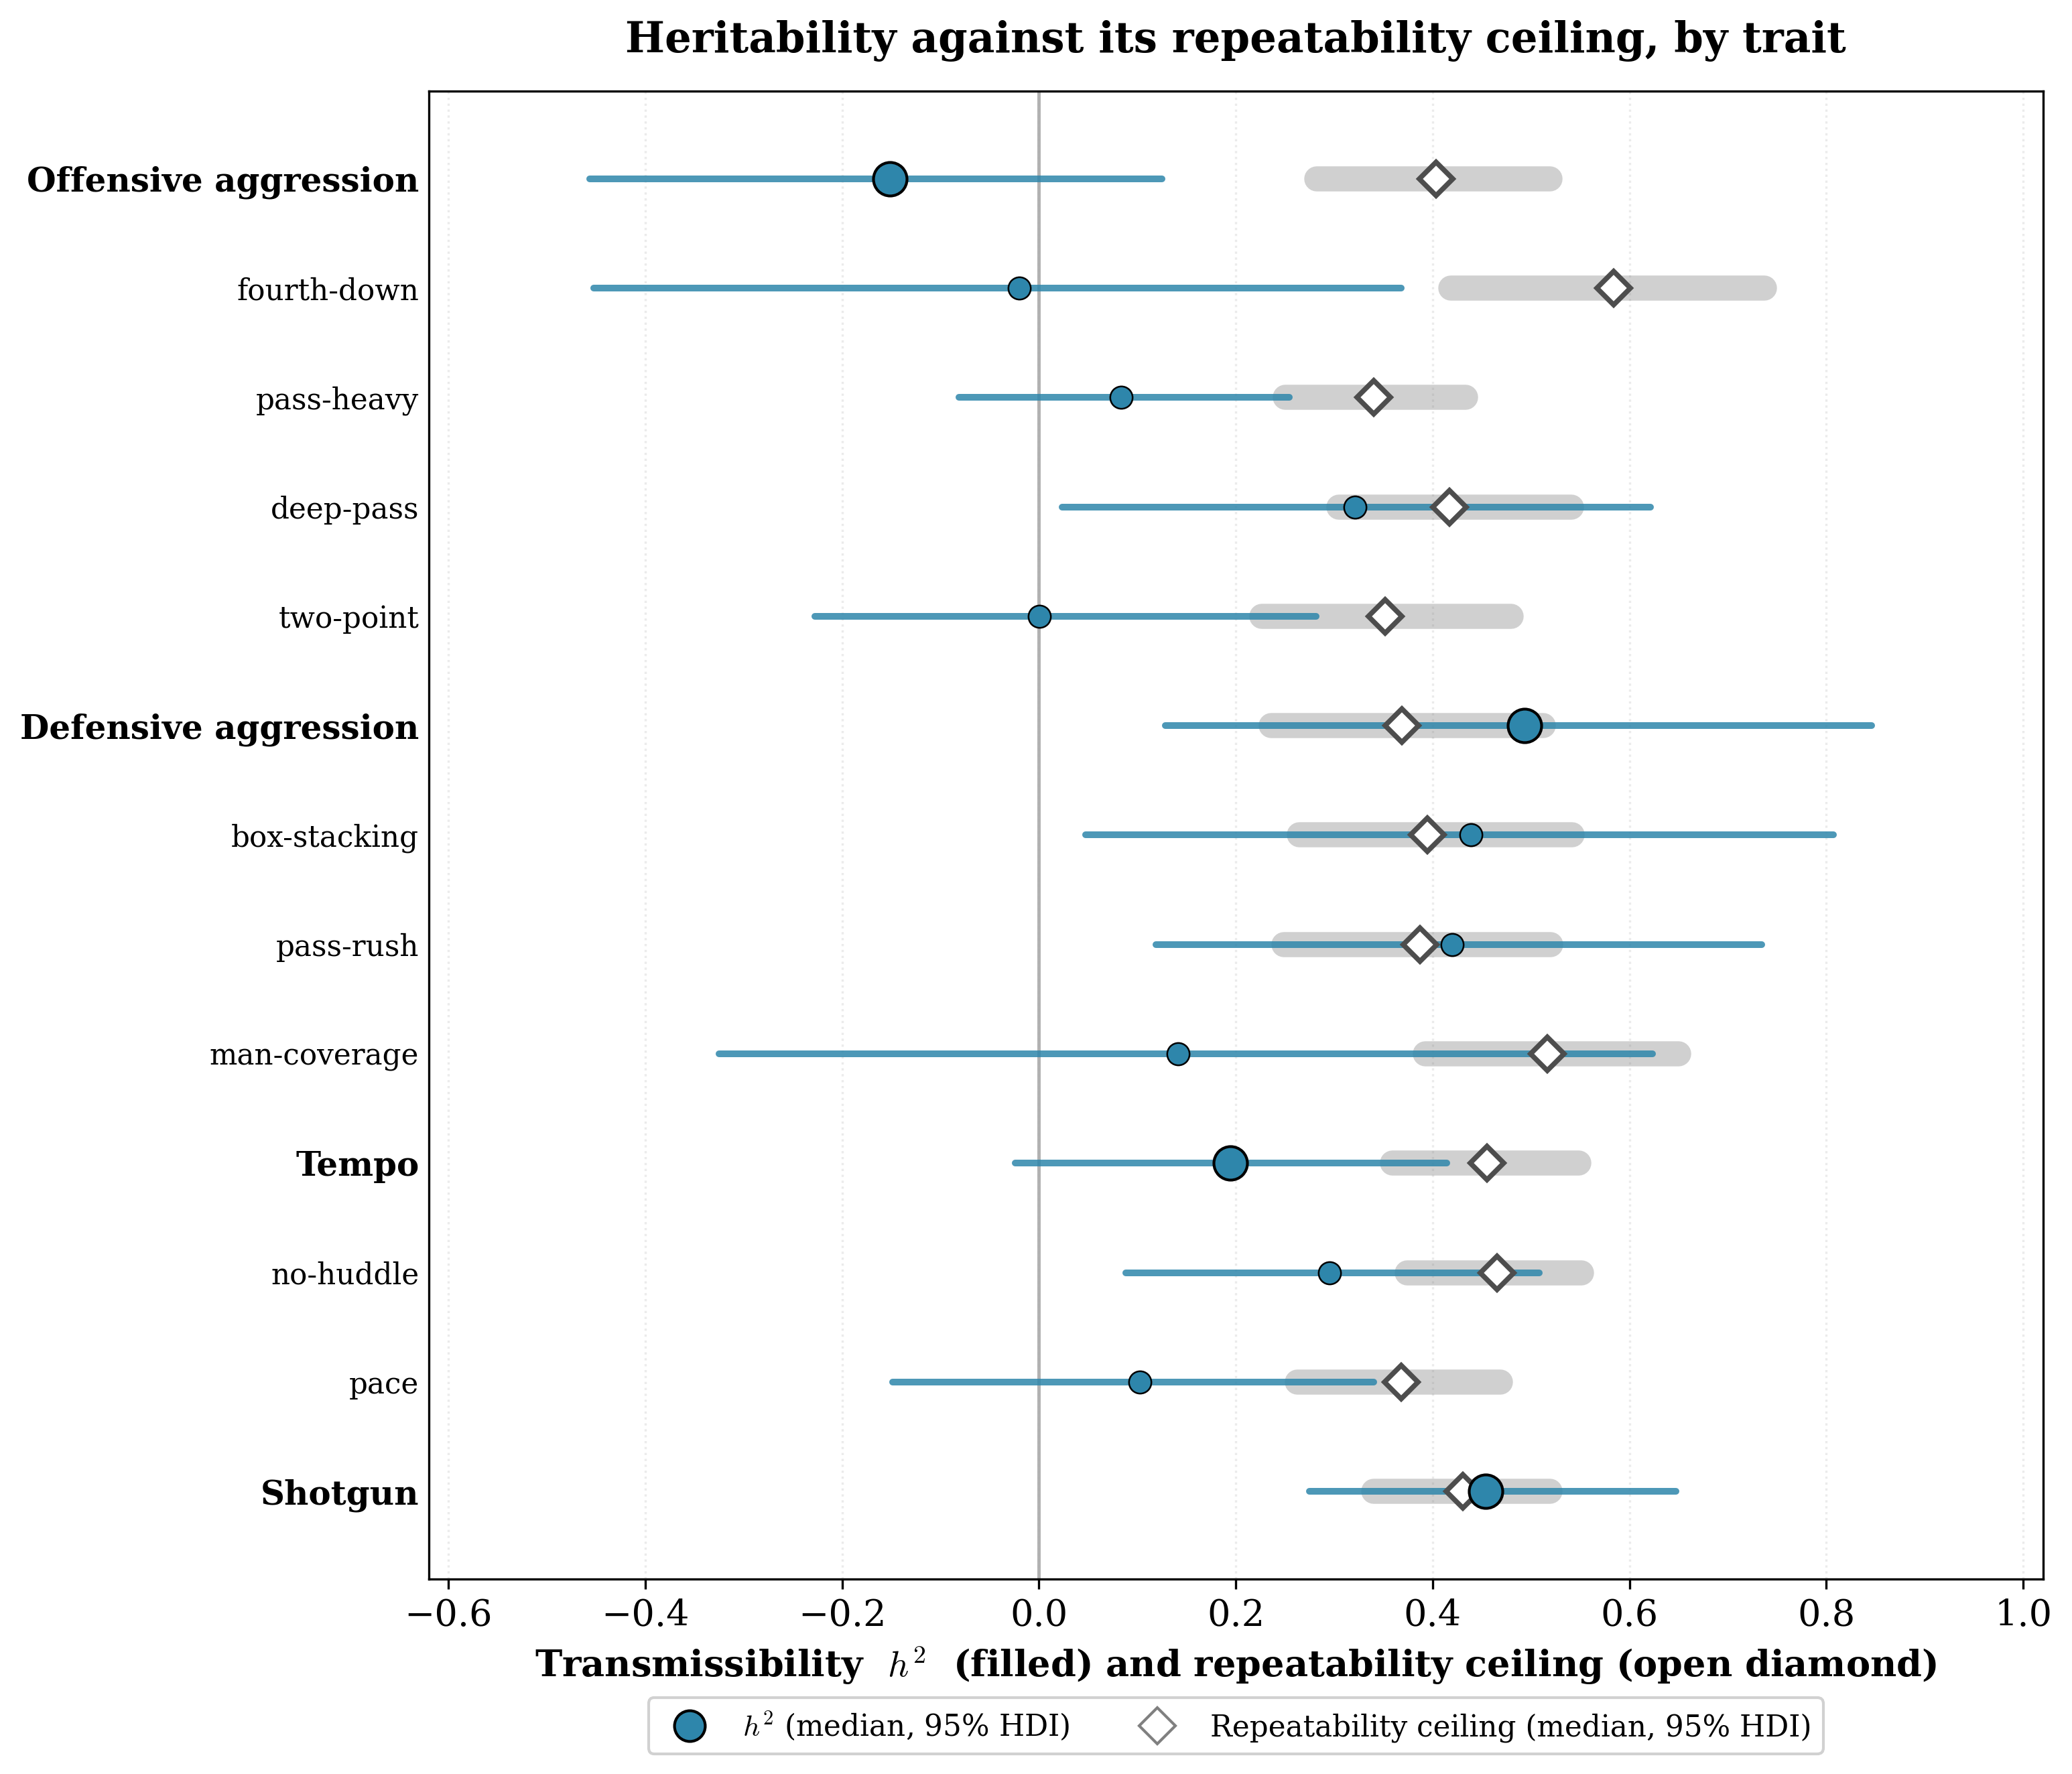
\includegraphics[width=0.92\textwidth]{../../visualizations/performance/ehs_heritability_forest.png}
\caption{Transmissibility ($h^{2}$, filled points with 95\% HDIs) against its
repeatability ceiling (open diamond, median; gray band, repeatability 95\% HDI) for
every trait, grouped by gene and colored by family. A heritability cannot exceed its
repeatability in the population; because $h^{2}$ and repeatability are estimated from
separate models with wide posteriors, their medians can cross for traits that
transmit near the ceiling, but every $h^{2}$ point falls within the repeatability's
credible interval (the posterior contrast $P(h^{2}>\text{repeatability})$ is 0.5 to
0.75 for these, that is $h^{2}\approx$ repeatability). Offensive aggression and its
components are repeatable but have $h^{2}$ indistinguishable from zero, a clean gap
($P=0.00$), the preregistered repeatable-but-not-heritable pattern (H2); schematic
identity and the defensive front transmit near their ceiling.}
\label{fig:forest}
\end{figure}

\begin{table}[t]
\centering
\caption{Transmissibility ($h^{2}$, C1), repeatability (C2), and selection ($S$)
for the four composites and the ten sub-traits. $h^{2}$ and repeatability are
posterior medians with 95\% HDIs; $S$ is the era-adjusted inverse-variance-weighted
correlation with WAR with a 95\% coach bootstrap CI. All C1/C2 fits met
$\hat{R}\le1.01$ and bulk ESS $>400$.}
\label{tab:main}
\begin{tabular}{llll}
\toprule
Trait & $h^{2}$ & repeatability & $S$ \\
\midrule
\textit{Offensive aggression} & $-0.15$ $[-0.46,0.12]$ & $0.40$ $[0.28,0.52]$ & $\phantom{-}0.18$ $[\phantom{-}0.08,0.27]$ \\
\quad fourth-down   & $-0.02$ $[-0.45,0.37]$ & $0.58$ $[0.42,0.74]$ & $\phantom{-}0.04$ $[-0.05,0.13]$ \\
\quad pass-heavy    & $\phantom{-}0.08$ $[-0.08,0.25]$ & $0.34$ $[0.25,0.43]$ & $\phantom{-}0.16$ $[\phantom{-}0.04,0.27]$ \\
\quad deep-pass     & $\phantom{-}0.32$ $[\phantom{-}0.02,0.62]$ & $0.42$ $[0.30,0.54]$ & $\phantom{-}0.09$ $[\phantom{-}0.00,0.17]$ \\
\quad two-point     & $\phantom{-}0.00$ $[-0.23,0.28]$ & $0.35$ $[0.23,0.48]$ & $-0.02$ $[-0.11,0.07]$ \\
\textit{Tempo}      & $\phantom{-}0.19$ $[-0.02,0.41]$ & $0.45$ $[0.36,0.55]$ & $\phantom{-}0.03$ $[-0.07,0.14]$ \\
\quad no-huddle     & $\phantom{-}0.30$ $[\phantom{-}0.09,0.51]$ & $0.47$ $[0.37,0.55]$ & $-0.02$ $[-0.11,0.08]$ \\
\quad pace          & $\phantom{-}0.10$ $[-0.15,0.34]$ & $0.37$ $[0.26,0.47]$ & $\phantom{-}0.07$ $[-0.04,0.19]$ \\
\textit{Defensive aggression} & $\phantom{-}0.49$ $[\phantom{-}0.13,0.85]$ & $0.37$ $[0.24,0.51]$ & $\phantom{-}0.15$ $[\phantom{-}0.03,0.27]$ \\
\quad box-stacking  & $\phantom{-}0.44$ $[\phantom{-}0.05,0.81]$ & $0.39$ $[0.26,0.54]$ & $\phantom{-}0.06$ $[-0.04,0.16]$ \\
\quad pass-rush     & $\phantom{-}0.42$ $[\phantom{-}0.12,0.73]$ & $0.39$ $[0.25,0.52]$ & $\phantom{-}0.17$ $[\phantom{-}0.04,0.29]$ \\
\quad man-coverage  & $\phantom{-}0.14$ $[-0.33,0.62]$ & $0.52$ $[0.39,0.65]$ & $\phantom{-}0.13$ $[-0.01,0.28]$ \\
\textit{Shotgun}    & $\phantom{-}0.45$ $[\phantom{-}0.27,0.65]$ & $0.43$ $[0.34,0.52]$ & $\phantom{-}0.08$ $[-0.03,0.17]$ \\
\bottomrule
\end{tabular}
\end{table}

\subsection{The heritability by selection map and the preregistered verdicts}
Placing the four composites in $h^{2}\times S$ space (Figure~\ref{fig:map}) makes
the structure visible. Offensive aggression sits in the adaptive-but-personal
corner (selected, not heritable); shotgun and tempo sit in the heritable-but-neutral
corner (transmitted, not selected); defensive aggression sits alone in the
adaptive-and-heritable corner. The two axes are close to orthogonal.

\begin{figure}[t]
\centering
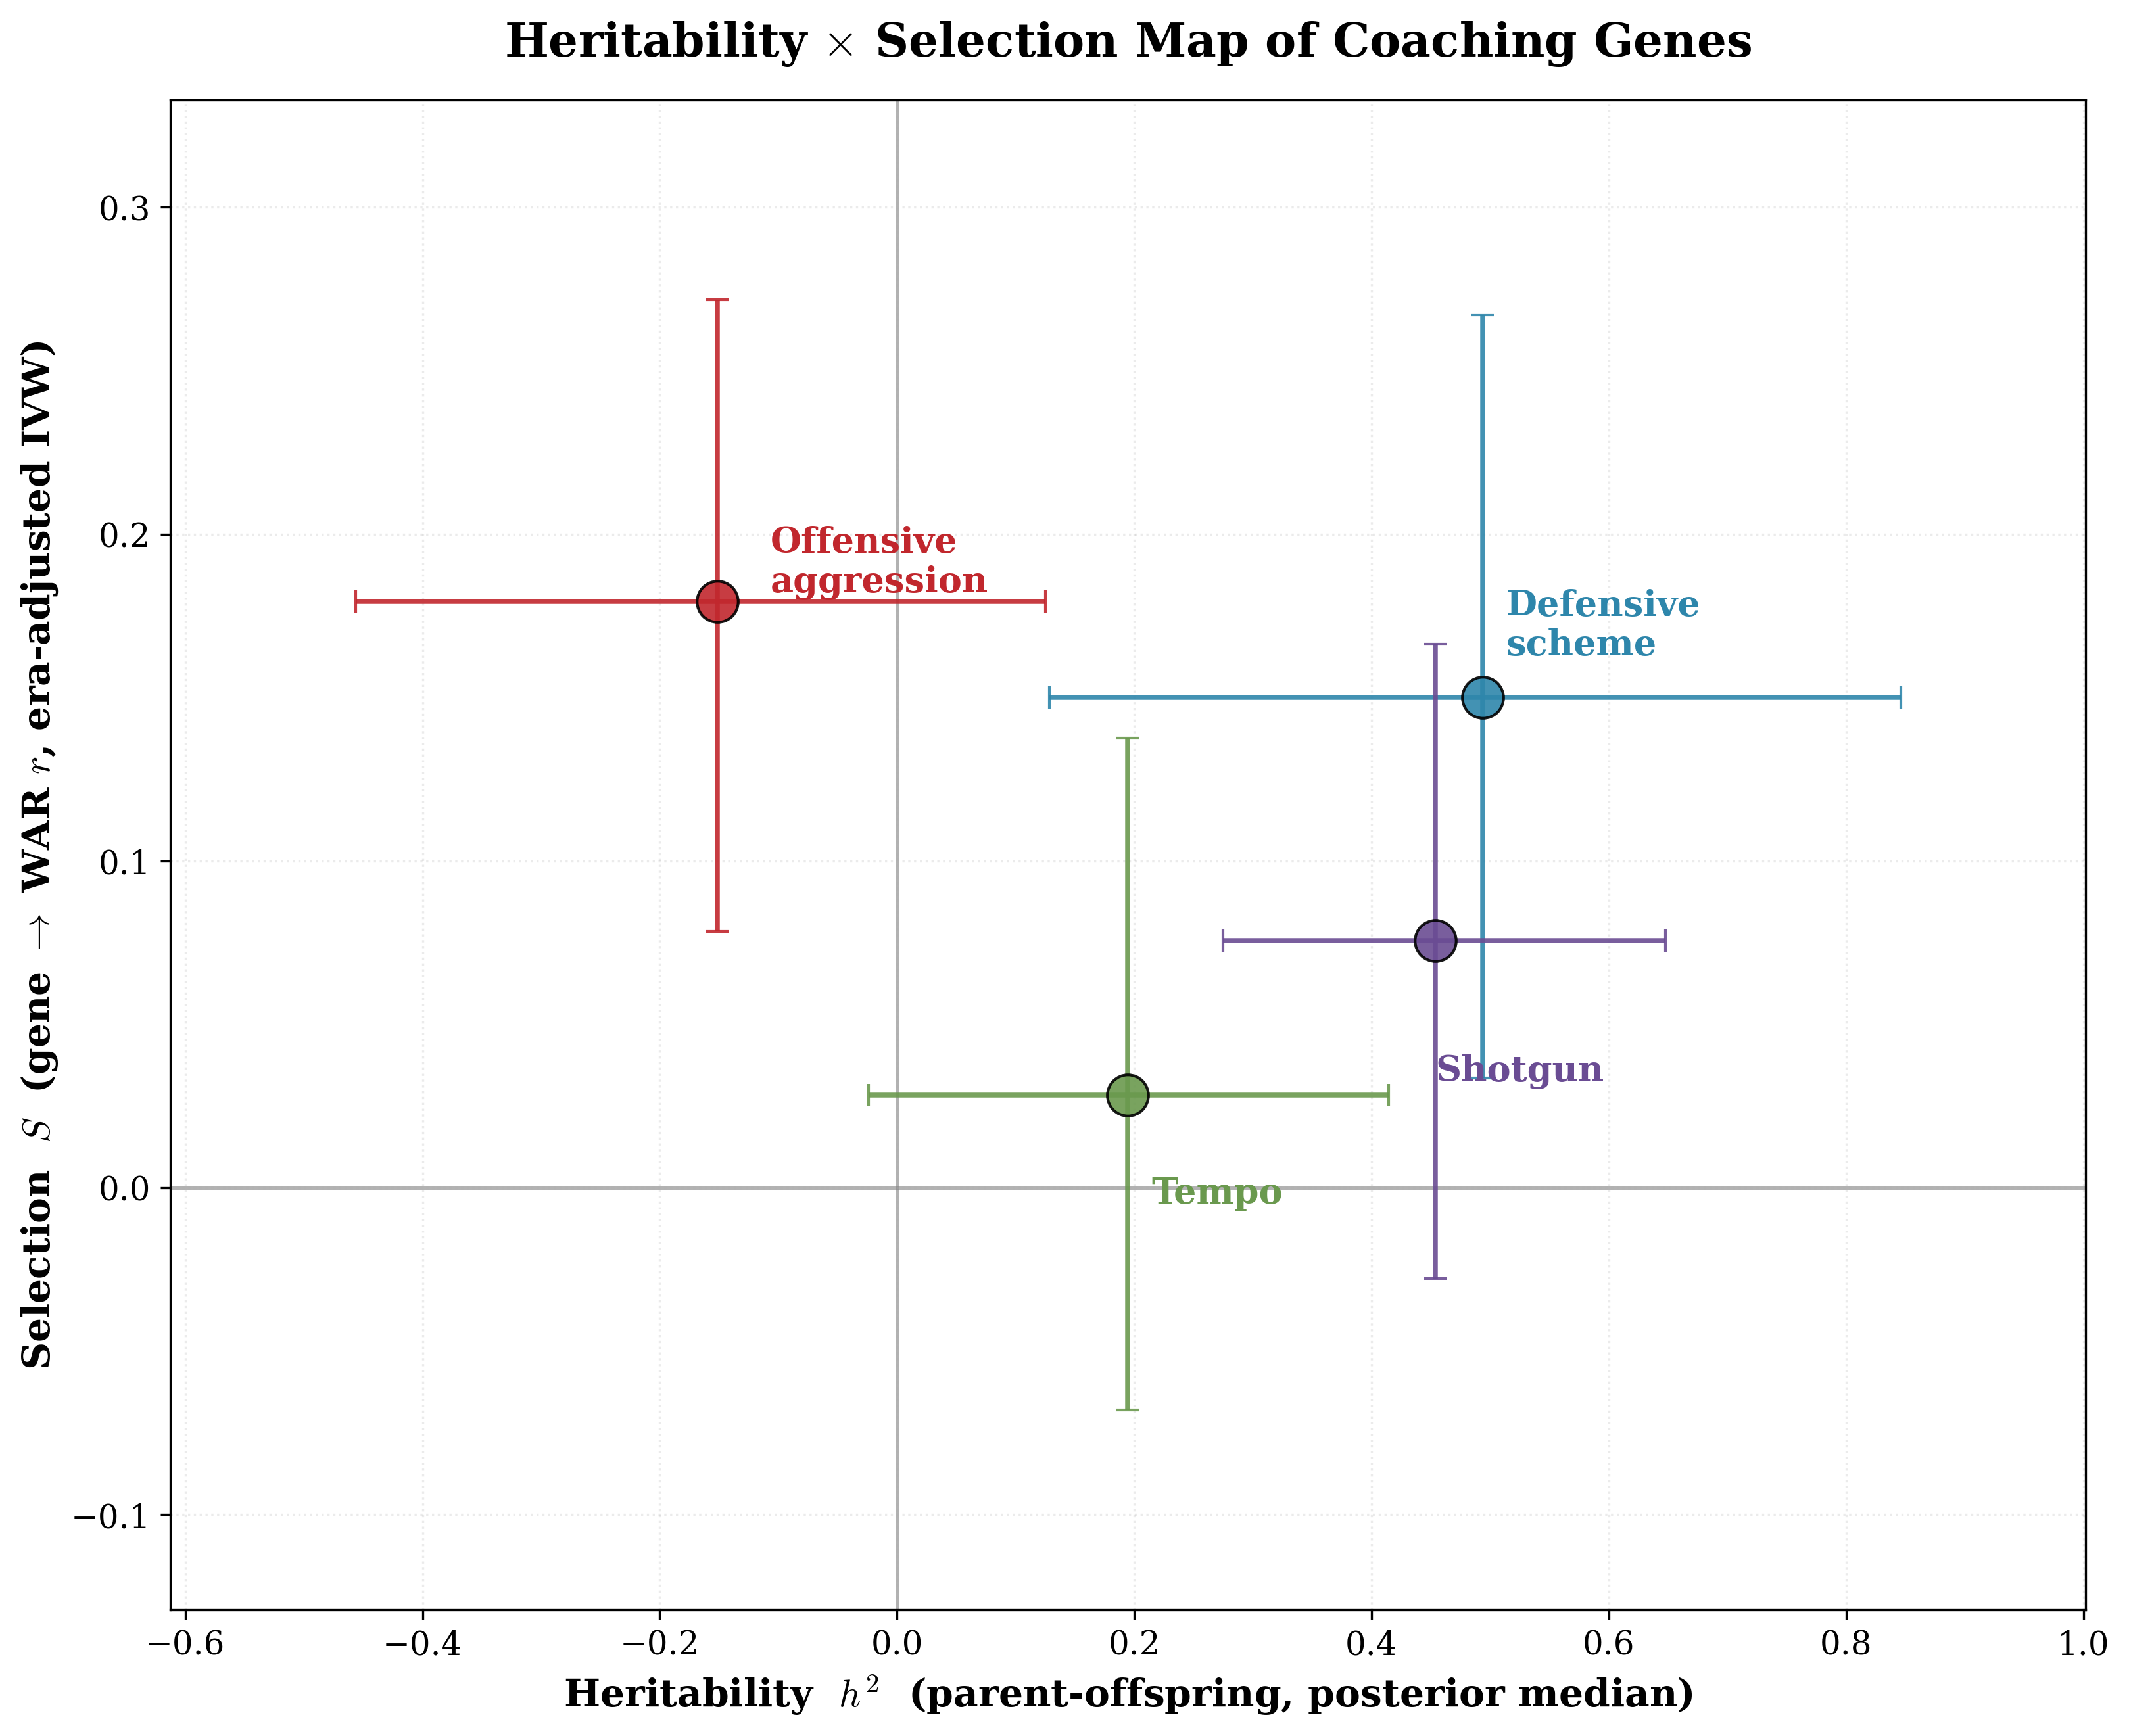
\includegraphics[width=0.86\textwidth]{../../visualizations/performance/gene_fitness_heritability_map.png}
\caption{Heritability ($h^{2}$, C1 posterior median) versus selection ($S$,
era-adjusted inverse-variance-weighted gene-WAR correlation) for the four
gene-level composites, with 95\% intervals on both axes. Offensive aggression is
adaptive but personal; shotgun and tempo are heritable but neutral; defensive
aggression is both. The axes are nearly independent.}
\label{fig:map}
\end{figure}

The three preregistered decision rules resolve as follows.

H2 is supported. Offensive aggression is repeatable ($0.40$) but not
heritable ($h^{2}=-0.15$); the preregistered contrast, repeatability minus $h^{2}$,
is $0.55$ with a 95\% HDI of $[0.24,0.87]$, excluding zero, and $P(h^{2}>\text{
repeatability})=0.00$. Offensive aggression is a real, stable, personal trait that
does not pass down the tree. The contrast behaves as the prereg intended
elsewhere too: for the traits that transmit near their ceiling (shotgun, defensive
aggression, box-stacking, pass-rush) $h^{2}$ and repeatability are statistically
indistinguishable ($P(h^{2}>\text{repeatability})$ between 0.5 and 0.75, each
$h^{2}$ inside the repeatability's credible interval), so the apparent crossings in
Figure~\ref{fig:forest} are estimation noise near the ceiling, not violations of the
bound.

H1 is not supported as a conjunction, though its selection half holds. The
approach family is more selected than the identity family (mean-$S$ difference
$+0.11$, 95\% interval $[0.01,0.22]$, excluding zero), but the identity family is
not reliably more heritable than the approach family (mean-$h^{2}$ difference
$+0.16$, $[-0.12,0.43]$, including zero). The heritability half fails for a
substantive reason: defensive aggression is an approach trait that is nonetheless
highly heritable ($h^{2}=0.49$), so the approach family does not have uniformly low
transmissibility. Whether defensive aggression is really a pure approach trait is
itself open to question: on defense the aggression measure blends a risk posture
(loading the box, sending rushers) with a scheme choice (man versus zone coverage),
so its high transmissibility may be the schematic half showing through rather than a
counterexample to the taxonomy. We take up this classification directly in
Section~\ref{sec:defagg}.

H3 is inconclusive. Across the ten sub-traits the Spearman correlation between
$h^{2}$ and $S$ is $+0.32$, but with a 95\% bootstrap interval of $[-0.54,0.69]$
(Figure~\ref{fig:scatter}) that runs from a strong negative to a strong positive
slope. The ten trait points form a broad cloud rather than a line, so many slopes
fit about equally well and the sign is not identified: a small change in the leverage
of any one trait would flip it, from the negative trade-off implied if offensive
aggression dominates to the positive relationship implied by the other three genes.
With so few traits the cross-trait test is underpowered, so we read the result as
uninformative about the sign rather than as evidence for or against a trade-off.

\begin{figure}[t]
\centering
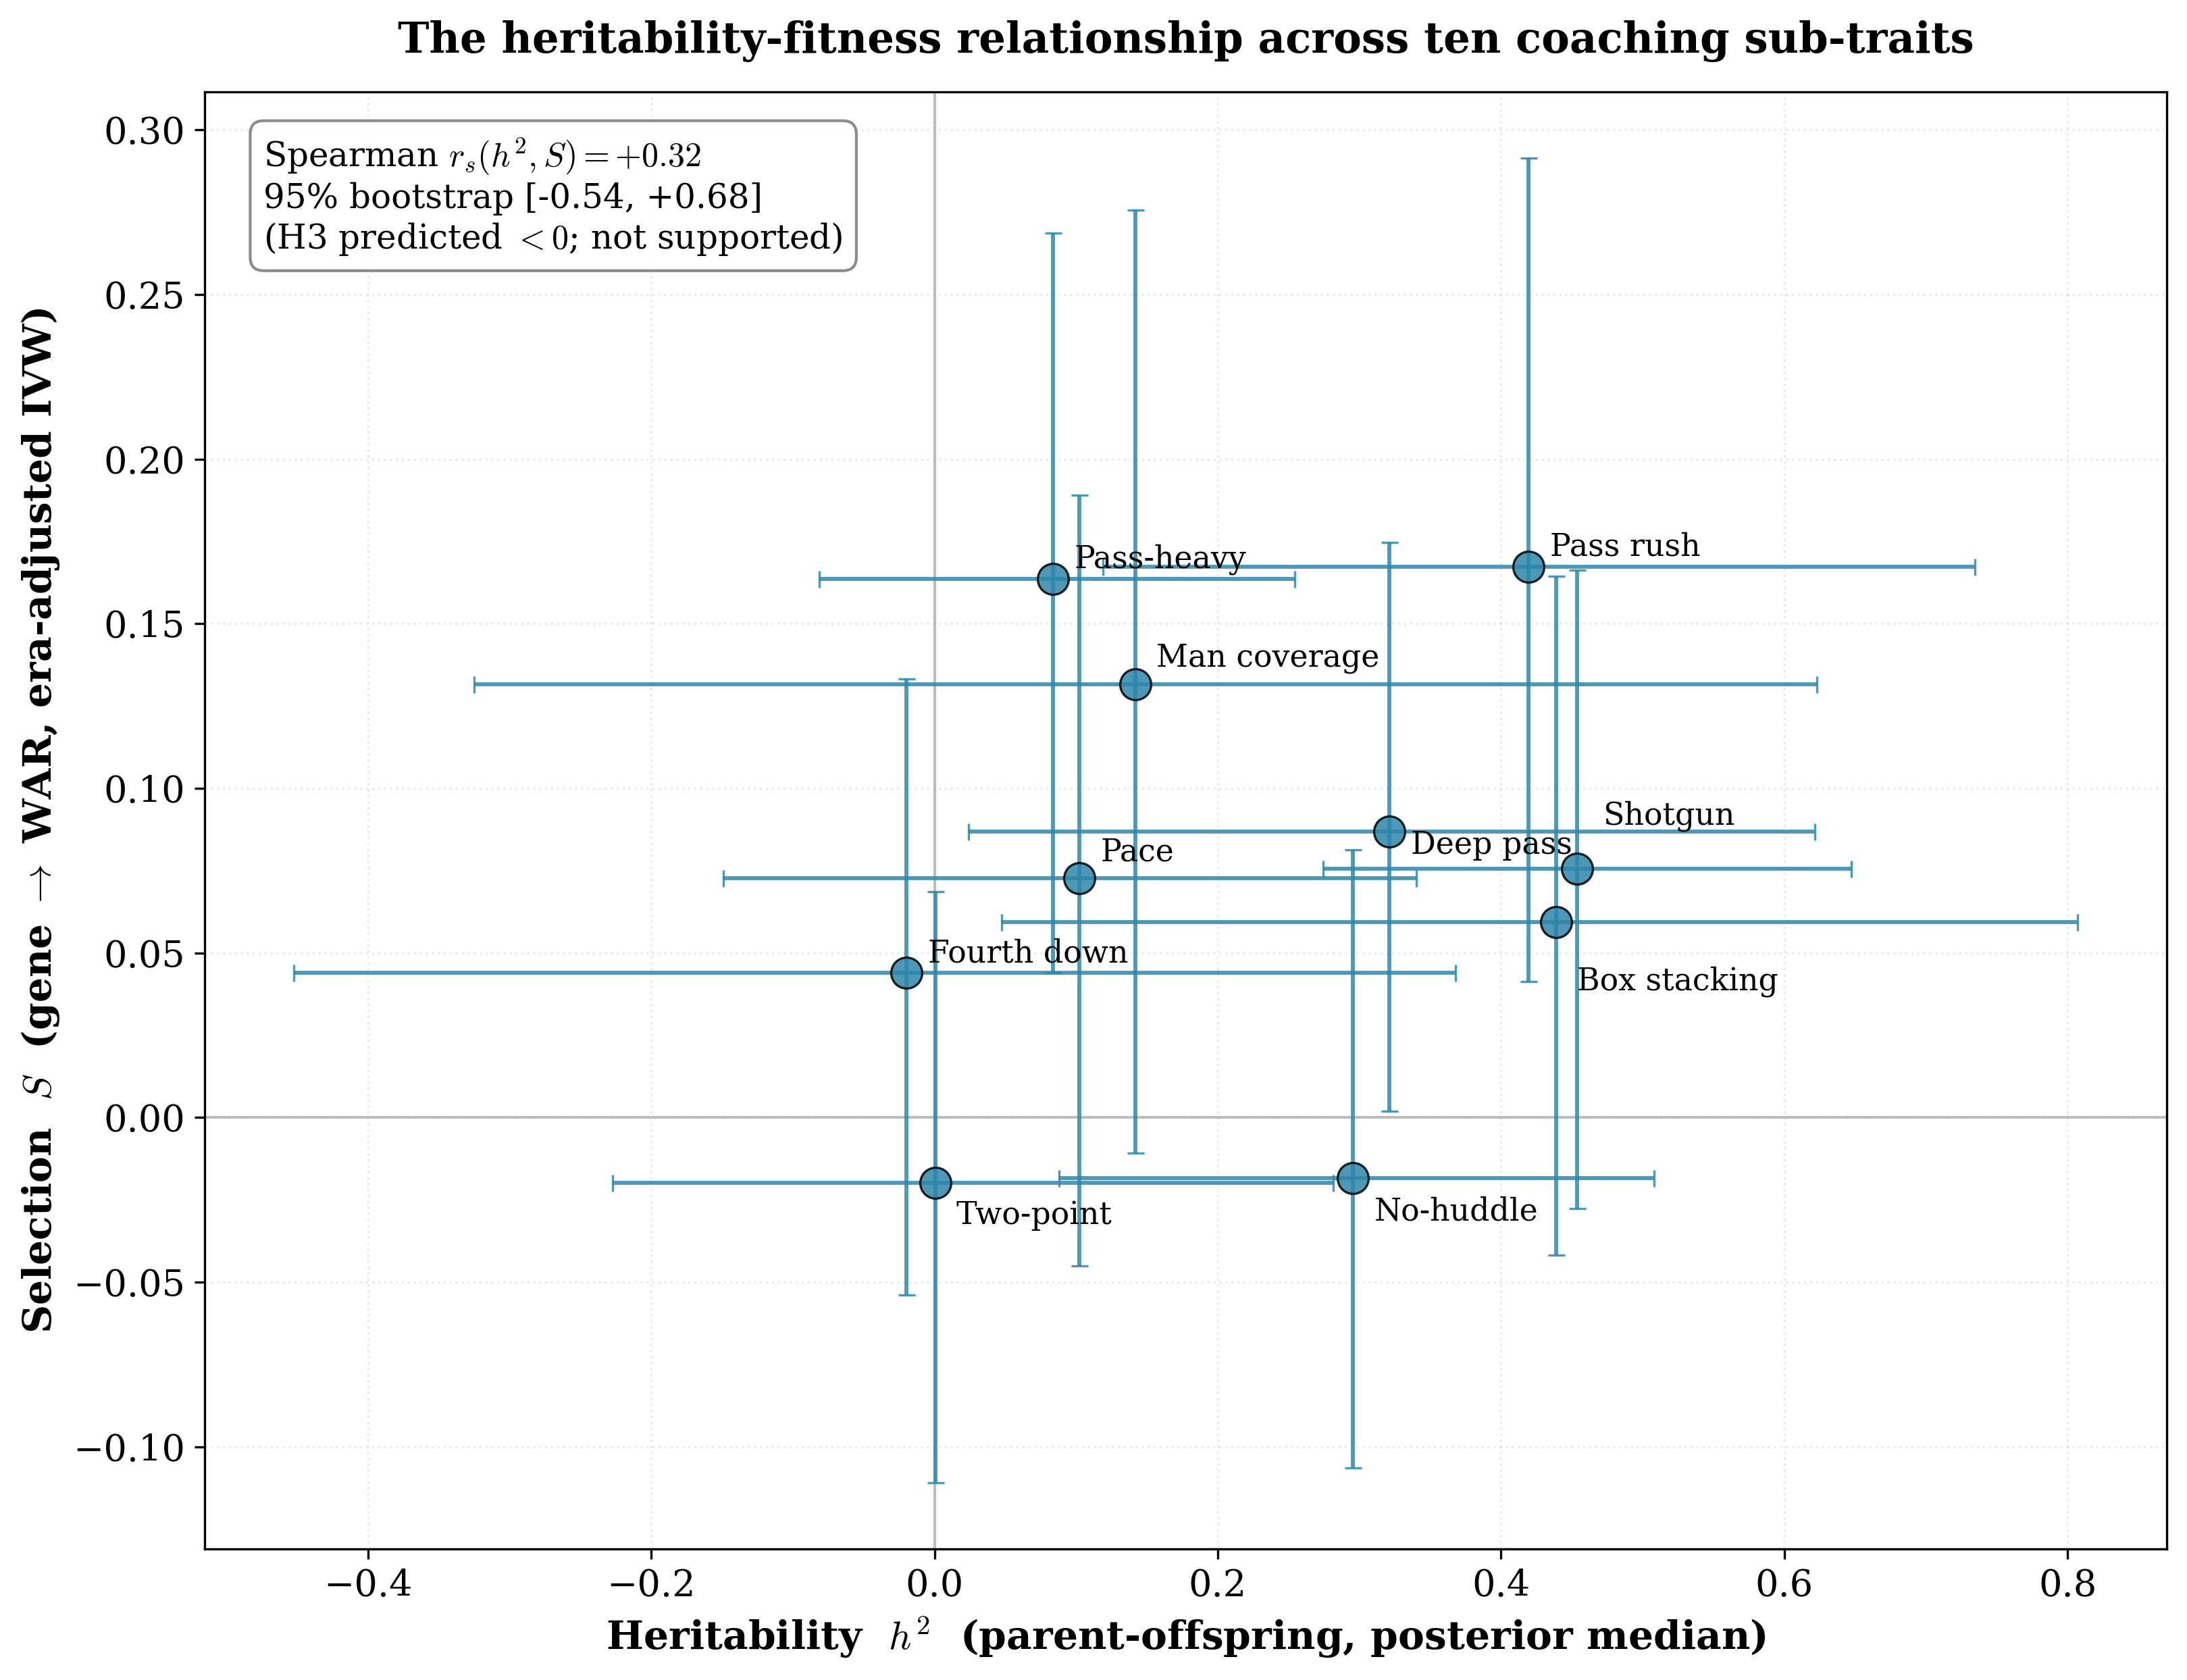
\includegraphics[width=0.9\textwidth]{../../visualizations/performance/ehs_cross_trait_h2_S.png}
\caption{The cross-trait heritability-fitness relationship, the cultural analog of
the wild-population test of \textcite{mousseauroff1987} and \textcite{kruuk2000}: each of
the ten sub-traits placed by transmissibility $h^{2}$ and selection $S$, with 95\%
intervals (a single colour throughout; the approach-versus-identity contrast is
drawn in the text, not by segmenting the figure). The Spearman rank correlation (H3)
is $+0.32$ ($[-0.54,0.69]$); the interval is too wide to fix the sign, so the
cross-trait trade-off test is inconclusive. The decoupling we describe rests on where
the traits sit in $h^{2}\times S$ space (Figure~\ref{fig:map}), not on this slope.}
\label{fig:scatter}
\end{figure}

Taken together, the verdicts describe a \emph{decoupling} rather than a trade-off.
Transmission and selection are close to independent across coaching traits, with
two clean archetypes, inherited-but-neutral identity (shotgun, tempo) and
selected-but-personal offensive aggression, and one trait, defensive aggression,
that occupies the both corner and is chiefly responsible for the absence of a clean
negative relationship.

\subsection{Exploratory: network signal, horizontal transmission, and reproductive
success}
Three exploratory analyses round out the picture; none is confirmatory. The first two
(network signal, reproductive rate) are corrected among themselves under a
Benjamini--Hochberg false-discovery rate; the third (horizontal transmission) is a
Bayesian model reported by posterior intervals, a separate family.

First, phylogenetic signal on the mentor network (Table~\ref{tab:moran},
Supplementary material). Moran's
$I$, the network analog of the tendency of related individuals to resemble one
another, is positive for the schematic and defensive genes and essentially zero for
offensive aggression (defensive aggression $I=0.21$, within-era permutation
$p=0.002$; tempo $0.12$, $p=0.008$; shotgun $0.08$, $p=0.04$; offensive aggression
$-0.01$, $p=0.52$). Under the exploratory correction the defensive and tempo signals
survive. The pattern mirrors the transmission results exactly: network-adjacent
coaches resemble one another in the traits that transmit and not in the trait that
does not, a second and independent line of evidence for the same decoupling.

Second, horizontal transmission, measured rather than inferred
(Figure~\ref{fig:horiz}). Holding a coach's own previous value and baseline fixed,
head coaches converge each season on the prevailing league level: pooled across the
ten sub-traits the convergence coefficient is $\mu_{\kappa}=0.22$ (95\% HDI
$[0.02,0.40]$, $P(\kappa>0)=0.98$). The pull is sharply selective and falls on exactly
the behaviors that swept the league: fourth-down aggression ($\kappa=0.57$, HDI
$[0.40,0.75]$), two-point attempts ($0.44$, $[0.24,0.64]$), deep passing ($0.32$,
$[0.04,0.60]$), the offensive-aggression composite ($0.37$, $[0.16,0.57]$), and
shotgun ($0.20$, $[0.09,0.30]$) all show credible convergence, while pace, no-huddle,
pass-heavy, and the defensive traits do not. This is the horizontal channel made
visible: fourth-down aggression, whose vertical $h^{2}$ is indistinguishable from
zero, is nonetheless pulled hard toward the league norm, the clearest case of a trait
that spreads across contemporaries rather than down lineages. Because conformity and
the drift it produces are nearly collinear, a model that also absorbs a per-trait
linear trend shrinks the pooled estimate to $0.05$ ($[-0.10,0.21]$); we therefore read
$\kappa$ as evidence that coaches converge on common norms, consistent with
frequency-biased social learning, while noting that convergence by peer imitation and
by a shared response to a changing environment are not fully separable here.

\begin{figure}[t]
\centering
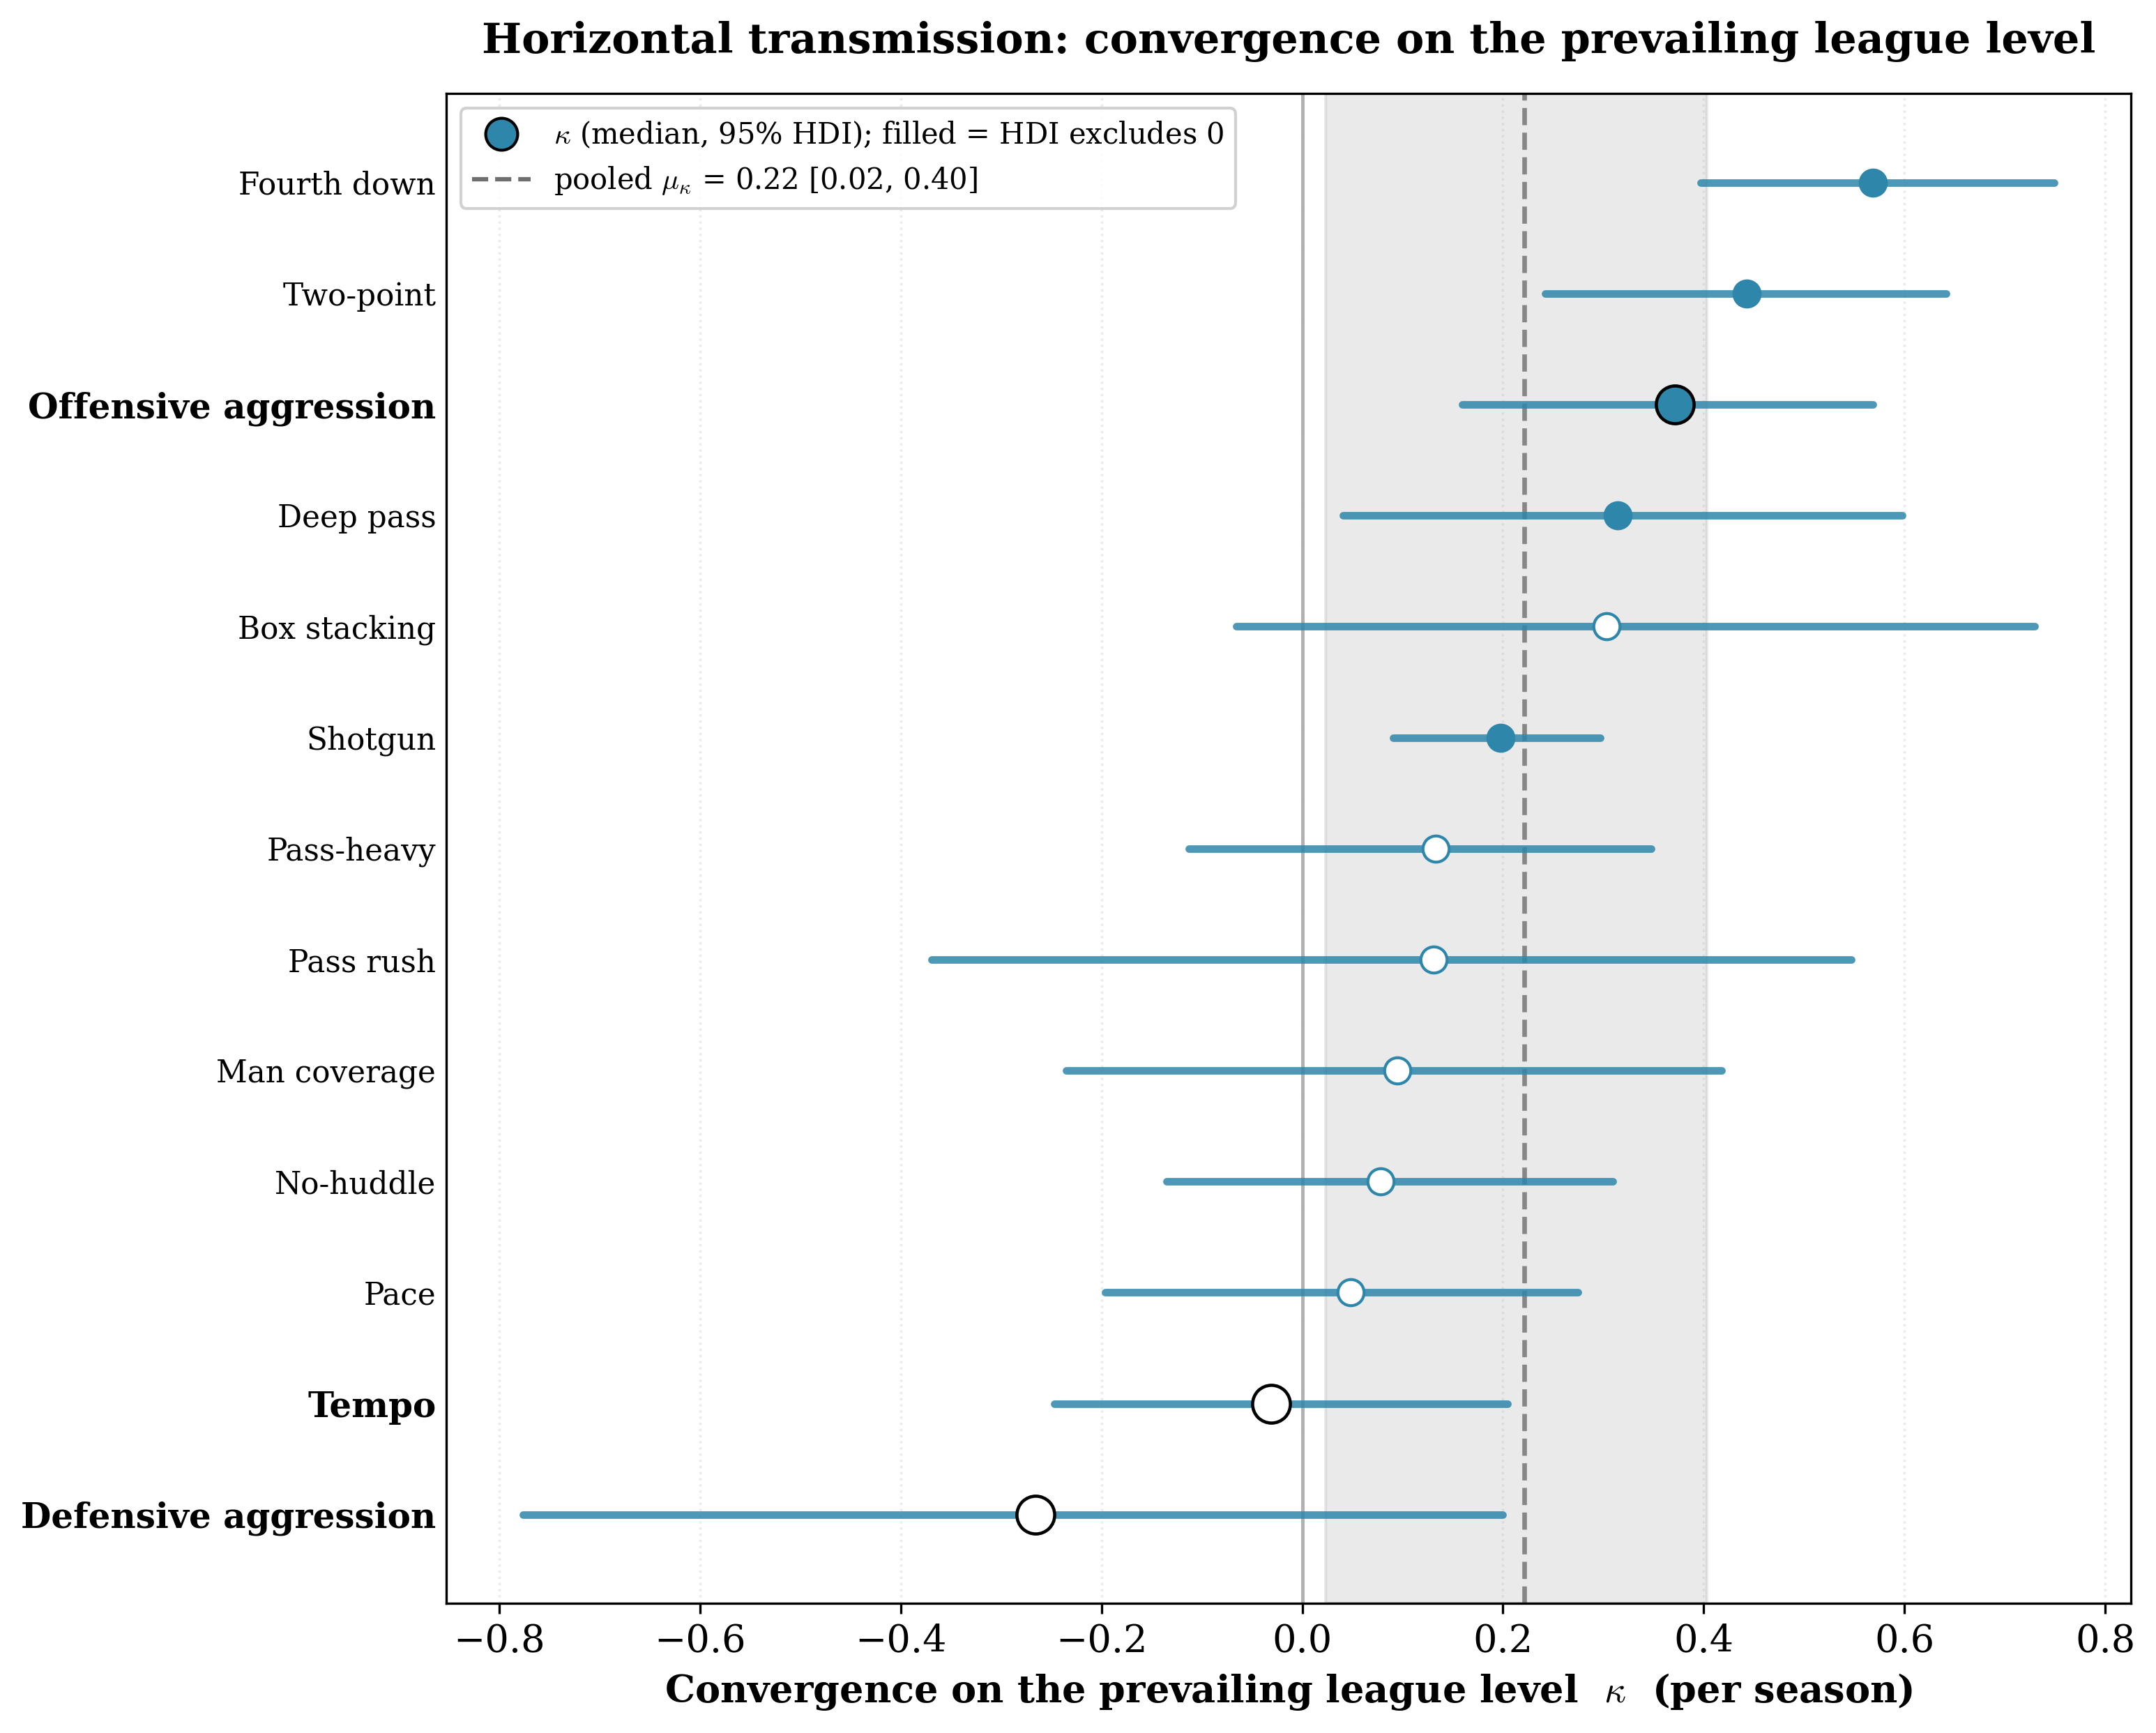
\includegraphics[width=0.9\textwidth]{../../visualizations/performance/horizontal_transmission_forest.png}
\caption{Horizontal transmission: per-trait convergence on the prevailing league
level ($\kappa$, posterior median and 95\% HDI) against the pooled estimate
$\mu_{\kappa}$ (dashed line and band). Filled markers have an HDI excluding zero.
Convergence is credible and largest for the behaviors that diffused across the league
(fourth-down, two-point, deep passing, the offensive-aggression composite, shotgun)
and absent for the traits that did not. The absolute (non-era-adjusted) phenotype is
used here so the league-wide drift is retained as the horizontal signal.}
\label{fig:horiz}
\end{figure}

Third, reproductive success, the other face of fitness (Figure~\ref{fig:repro}).
Counting a mentor's distinct proteges who themselves became head coaches, the
distribution is heavy-tailed: across 265 modern-era head coaches (first head-coaching
season in 1970 or later, matching the post-merger era) the Gini coefficient is 0.56
and the most prolific decile produced 35\% of all head-coaching descendants, with
Marty Schottenheimer and Bill Parcells (13 each), Bill Belichick (12), and Andy Reid
(11) at the top. Reproductive success tracks career WAR ($r=0.35$), but the link runs
through longevity rather than per-season quality: offspring count correlates 0.74
with seasons coached, and net of tenure the exposure-normalized rate (offspring per
head-coaching season) is essentially unrelated to quality (partial $r=0.07$). A
coach's ecological fitness (winning) and reproductive fitness (descendants) are thus
only weakly linked, and through survival: coaches shape the league less by winning in
any given season than by lasting long enough to send many proteges into
head-coaching chairs, carrying their schematic identity, though not their competitive
edge, with them.

\begin{figure}[t]
\centering
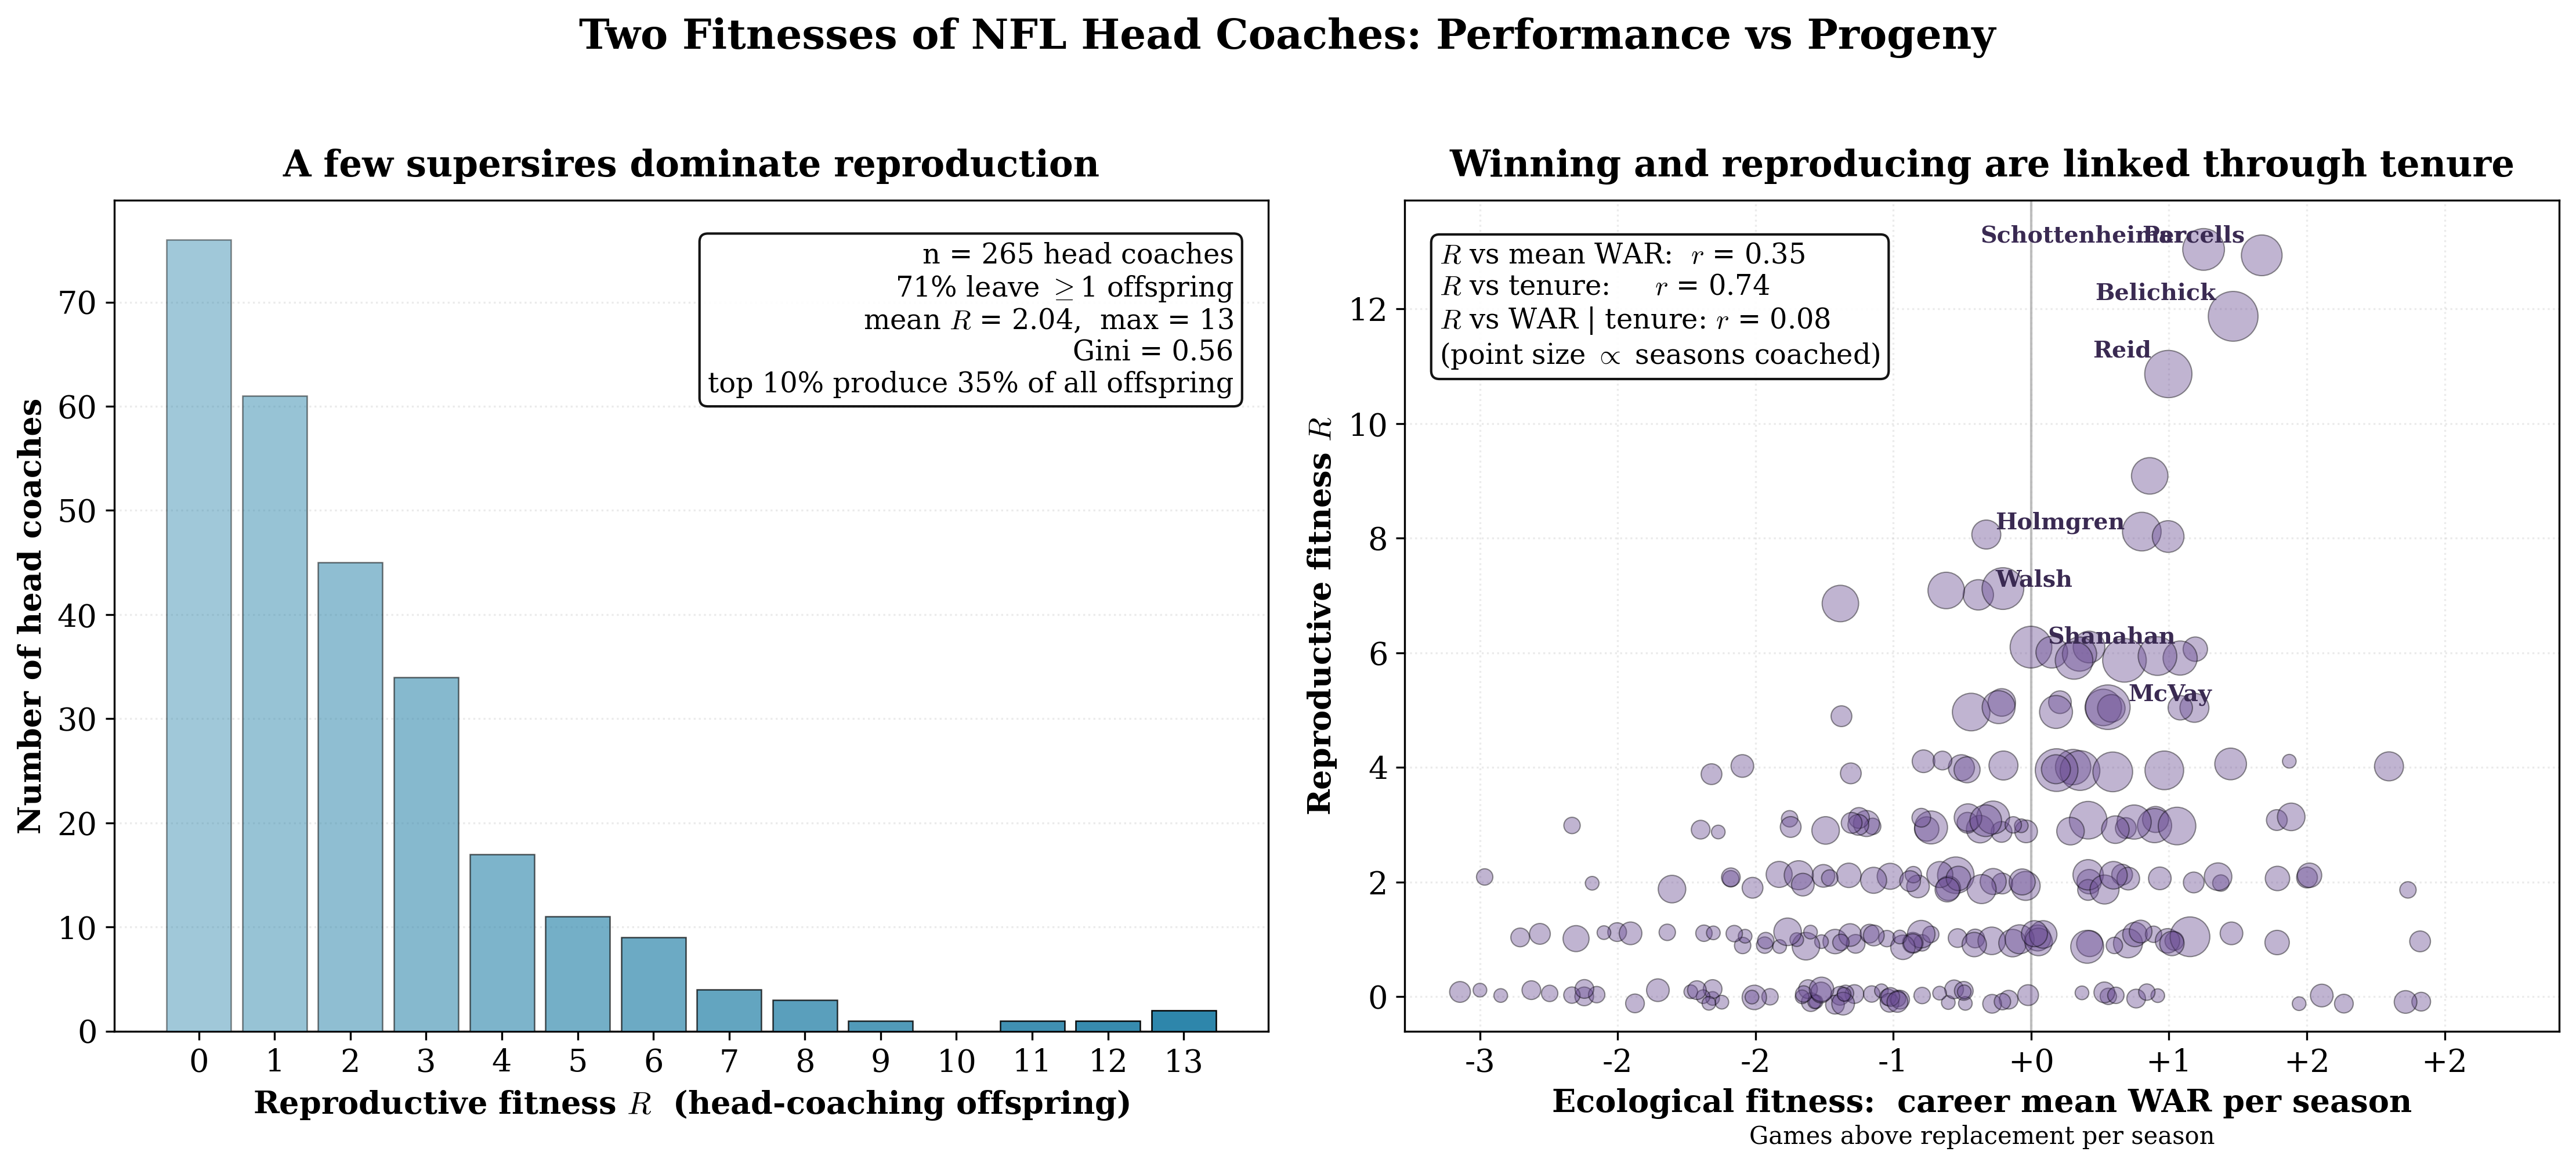
\includegraphics[width=0.92\textwidth]{../../visualizations/performance/reproductive_fitness.png}
\caption{Two fitnesses of NFL head coaches. Left: the distribution of reproductive
fitness (number of head-coaching proteges) is heavy-tailed (Gini 0.56; top decile
produces 35\% of all descendants). Right: ecological fitness (career mean WAR per
season) versus reproductive fitness, point size proportional to seasons coached; the
positive raw association ($r=0.35$) is carried by tenure (offspring versus seasons
coached $r=0.74$), and net of tenure quality barely predicts offspring (partial
$r=0.07$).}
\label{fig:repro}
\end{figure}

%% ----------------------------------------------------------------------------
\section{Discussion}
%% ----------------------------------------------------------------------------

\subsection{Decoupling, not a trade-off}
We set out to test whether the traits that transmit down a coaching lineage are the
traits that win, expecting the negative heritability-fitness relationship familiar
from biological populations. That specific trade-off did not appear, but neither
did any clear relationship in the other direction: with so few traits the
$h^{2}$-by-$S$ association is indeterminate (cross-trait Spearman $+0.32$ across the
ten sub-traits, interval spanning zero). The traits scatter in a loose square rather
than along a line, and the estimate is held back from being negative chiefly by
defensive aggression, the single trait that sits in the both-corner. We therefore do
not read the cross-trait slope as a structure in its own right. What is interpretable
is where individual traits fall in the $h^{2}$-by-$S$ plane, and there two archetypes
are clean. Schematic-identity traits,
shotgun and tempo, are transmitted faithfully ($h^{2}$ up to $0.45$) yet carry no
detectable fitness consequence ($S\approx0$): in evolutionary terms they behave
like heritable but selectively neutral markers \parencite{kimura1968}, tags of lineage
that ride along with apprenticeship rather than with winning. Offensive aggression
is the mirror image, a repeatable and selected but non-transmitted trait ($h^{2}$
indistinguishable from zero, $S=0.18$): among the offensive traits we measured, the
one that predicts success, in-game aggression, is a personal characteristic that
does not pass down. This last pattern is the preregistered H2,
and it is the sharpest single result: a trait can be a stable individual property
(repeatability $0.40$) and predict success and still not be inherited.

We preregistered a negative relationship and did not find one. That null invites a
sharper reading through the breeder's equation, $R=h^{2}S$, which gives a trait's
per-generation response to selection along a lineage. For offensive aggression the
lineage prediction is essentially nil ($R\approx h^{2}S\approx 0\times 0.18=0$),
because the trait is not transmitted, and yet its league-wide mean rose steadily
over our window. A quantity that the breeder's equation says should barely change
down the tree changed markedly across the population, the empirical signature that a
second, non-vertical channel is at work.

\subsection{Two channels: vertical down the tree, horizontal across the league}
The classical trade-off assumes a single inheritance channel along which selection
erodes heritable variance. Coaching has two such channels \parencite{cavallisforza1981,
boydricherson1985}. The schematic-identity traits spread \emph{vertically}, down the
offensive-coordinator apprenticeship. Shotgun shows this most clearly, with a
parent-offspring $h^{2}$ of $0.45$ whose interval excludes zero; tempo points the
same way, with a positive $h^{2}$ ($0.19$) and a within-era network signal that
survives correction (Table~\ref{tab:moran}). Offensive aggression, lacking a vertical channel
($h^{2}\approx0$, no network autocorrelation), spread \emph{horizontally} instead.
Its league-wide mean rose monotonically across our window (linear trend $r=0.91$ with
season, $p<0.001$; a large early-to-late shift, Cohen's $d=5.4$), crossing from below
the time-invariant, season-agnostic baseline in the late 2000s to clearly above it by
the early 2020s: the classic profile of a payoff-driven innovation copied among
contemporaries. Because the expectation model excludes season, that drift is genuine
change in behavior rather than a modeling artifact; with no vertical pathway to carry
it, that drift is horizontal spread among contemporaries, which we now measure rather
than only infer. Holding a coach's own history fixed, head coaches converge each
season on the prevailing league level, credibly so for fourth-down aggression and the
other behaviors that swept the league (Figure~\ref{fig:horiz}); fourth-down
aggression, with $h^{2}$ at zero, is pulled hardest of all. That convergence is the
footprint of frequency-biased copying, though imitation and a shared response to a
changing environment cannot be fully separated in it.

This is where the study answers the questions its predecessor left open.
\textcite{mesoudi2020} showed that football managers choose formations by strategic
social learning, weighting their own and the wider population's recent use of a
tactic, so that a successful formation diffuses horizontally as managers copy it from
their peers; and he named two channels his data could not reach, transmission down
mentor--protege lineages and the flow of influence along the network ties between
managers, illustrated by the lineage of managers who carry Bielsa's approach. Our
design adds the channel his could not reach. The mentor--protege $h^{2}$ slopes, and
the Moran's $I$ on the same apprenticeship network (Table~\ref{tab:moran}), put
numbers on the lineage transmission he pointed to but could not measure; both,
however, describe the vertical channel, not the peer ties he named. The horizontal
channel is more his than ours: he modeled peer copying directly, from
formation-adoption dynamics, whereas we measure only its aggregate footprint, the
season-by-season convergence of coaches on the prevailing norm
(Figure~\ref{fig:horiz}), not the dyadic copying itself. With that asymmetry stated,
the two studies interlock. The trait
Mesoudi's horizontal lens tracks, the fitness-linked one, is exactly the trait our
vertical lens finds absent from the coaching tree; the trait our vertical lens finds
transmitting is not the one that sweeps the league on a fitness gradient. Vertical
transmission carries system identity; horizontal transmission carries the winning
tactic. A study looking only down the tree would conclude aggression is absent from
coaching culture; a study looking only at league-wide diffusion would miss that
scheme is inherited.
Read together, the two channels partition the strategic repertoire, and the era
structure we remove as a statistical confounder is, substantively, the horizontal
channel itself.

\subsection{Defensive aggression: attitude and scheme entangled}
\label{sec:defagg}
Defensive aggression is the one composite that both transmits ($h^{2}=0.49$) and
predicts winning ($S=0.15$), and it is chiefly why the cross-trait relationship is
not cleanly negative. It is best read not as a counterexample but as a reminder that
our two-family taxonomy, approach versus identity, is cleaner on offense than on
defense. ``Aggression'' on defense bundles dimensions the offensive split holds apart, and
they differ in how schematic they are. The number of pass rushers, for one, is as
much a schematic property as an attitudinal one: whether a front rushes four or five
is largely a matter of running a 4--3 or a 3--4 base, not a play-by-play risk
decision, and box-stacking is similarly tied to front and personnel. Man versus zone
is the least schematic of the three, closer to a situational, matchup-driven call.
Transmissibility follows that ordering: box-stacking and pass-rush transmit strongly
($h^{2}=0.44$ and $0.42$), like schematic identity, while man coverage transmits
weakly ($h^{2}=0.14$). A composite that folds these together inherits transmissibility
from its schematic components and a fitness link from its aggressive posture, which is
precisely the both-corner position it occupies. The organizing distinction is attitude
versus scheme rather than offense versus defense, and on defense the two are entangled
within a single composite; a cleaner future decomposition would separate a defense's
situational risk posture from its base front and coverage system.

\subsection{Coaching lineages transmit systems, not success}
A common rationale for hiring from established coaching trees is that success flows
from mentor to protege. That claim finds little support here: working under a
successful mentor does not predict a protege's own success (mentor-protege WAR resemblance $r=0.12$, 95\% CI
$[-0.01,0.26]$, mentor-clustered $p=0.07$; $n=192$ pairs across 87 mentors, not
distinguishable from zero), and the in-game risk tendency that does predict success
is not passed down. What coaching trees
reliably transmit is schematic system, formation and tempo identity, and
specifically through the coordinator who would install it. There is a labor-market
reading of this asymmetry: an organization can observe and verify the system a
coordinator runs far more readily than whether he will win, so hiring on visible
schematic pedigree is hiring on the trait that transmits, not the trait that drives
value. What is legible (system) and what is decisive (in-game approach) come apart,
and only the former leaves a lineage to point to. We offer this as interpretation
rather than a tested claim; the confirmatory result is the decoupling itself.

\subsection{Limitations}
The transmission samples are small (40 offensive and 17 defensive
coordinator-to-head-coach transitions, and only 12 for man coverage), so the $h^{2}$
posteriors are wide and the
cross-trait test in particular has low power; H3's wide interval should be read as
inconclusive about a weak relationship, not as evidence for a positive one.
Coaching staffs are groups, but our transmission model reduces each to the single
head-coach-to-coordinator (OC or DC) link we can measure; position coaches, multiple
simultaneous coordinators, and overlapping staffs, the real structure of a coaching
tree, are simplified away. The genes attribute team play-calling to the head
coach and do not isolate a coordinator's individual contribution; the transmission
tests therefore ask whether the head-coaching style a coach apprenticed under
predicts his own later style, a mentor-protege resemblance that is consistent with
social learning but cannot, on its own, be separated from assortative hiring, in
which head coaches recruit coordinators who already share their approach.
Distinguishing the two would take a phenotype measured before the apprenticeship, or
staffs assigned rather than chosen; neither is generally available, since a coach's
play-calling style is not defined until he runs a unit. We therefore read $h^{2}$ as
vertical transmissibility in the broad sense. The
defensive-aggression measures begin in 2016 and man coverage in 2018, and the
defensive-aggression to WAR link may partly reflect reverse causation (better
defensive talent enables man coverage and extra rushers). Finally, single-season
WAR is noisy; we address this with inverse-variance weighting and treat the
season-level estimates as conservative floors. One asymmetry in evidential status
follows from the design: our mentor network encodes documented apprenticeship ties
rather than the full web of peer influence among contemporaries, so the vertical
channel is estimated directly, from both measured endpoints, while the horizontal
channel is measured only as aggregate convergence on the league norm, not as the
dyadic peer copying that \textcite{mesoudi2020} modeled directly; convergence by
imitation and by a shared response to a changing environment are not fully separable
in our data.

\subsection{Conclusion}
Treating the NFL coaching tree as a cultural pedigree, we find that the strategic
traits that transmit are largely not the traits that win. Schematic identity is
inherited but neutral; offensive aggression is selected but personal and,
strikingly, not heritable despite being a stable individual trait; defensive
aggression alone both transmits and wins. The negative heritability-fitness
relationship of biological populations does not appear; transmission and selection
are instead decoupled, and the fitness-linked behavior spreads horizontally rather
than down the lineage. Coaching trees, in the end, propagate systems, not success.

%% ----------------------------------------------------------------------------
\section*{Supplementary material}

\begin{table}[h]
\centering
\caption{Within-era phylogenetic signal on the mentor network (Moran's $I$ on a
row-normalized, undirected adjacency of mentor--protege ties; one-sided permutation
$p$ from within-career-midpoint-era label shuffles). $E[I]=-1/(N-1)$ is the
no-signal expectation. Under the exploratory Benjamini--Hochberg correction the
defensive-aggression and tempo signals survive.}
\label{tab:moran}
\begin{tabular}{lcccccc}
\toprule
Gene & $I$ & $E[I]$ & $z$ & $p$ & $N$ & edges \\
\midrule
Offensive aggression & $-0.01$ & $-0.01$ & $-0.04$ & 0.52 & 139 & 440 \\
Shotgun & $+0.08$ & $-0.01$ & $+1.77$ & 0.04 & 139 & 440 \\
Tempo & $+0.12$ & $-0.01$ & $+2.63$ & 0.008 & 139 & 440 \\
Defensive aggression & $+0.21$ & $-0.01$ & $+3.03$ & 0.002 & 95 & 216 \\
\bottomrule
\end{tabular}
\end{table}

%% ----------------------------------------------------------------------------

\paragraph{Acknowledgments}
This work uses play-by-play data from \texttt{nfl\_data\_py} and coaching histories
from Pro Football Reference; the WAR phenotype is from a companion
wins-above-replacement project.

\paragraph{Funding Statement}
This research received no specific grant from any funding agency, commercial or
not-for-profit sectors.

\paragraph{Competing Interests}
The author declares none.

\paragraph{Data Availability Statement}
\ifblind
The confirmatory analyses (C1--C3, hypotheses H1--H3) were preregistered before any
confirmatory quantity was computed on the final measurement pipeline. All data and
analysis code are public and seed-fixed, and the full pipeline runs from a single
command; the preregistration, data, and code repository links are withheld here to
preserve author anonymity and will be provided on acceptance.
\else
The confirmatory analyses (C1--C3, hypotheses H1--H3) were preregistered before any
confirmatory quantity was computed on the final measurement pipeline:
\url{https://doi.org/10.17605/OSF.IO/Y2KR5} (osf.io/y2kr5). All data and analysis
code are public and seed-fixed, and the full pipeline runs from a single command:
\url{https://github.com/jwilliamson7/Coach_Tree}. The WAR phenotype is drawn from
the sibling repository \url{https://github.com/jwilliamson7/Coach_WAR}, pinned at
commit \texttt{dffe2f1}.
\fi

\paragraph{Ethical Standards}
The research uses only publicly available data on professional-sport outcomes and
involves no human or animal subjects; it meets all applicable ethical guidelines.

\paragraph{Author Contributions}
J.W. conceived the study, developed the methods and software, conducted the
analysis, produced the visualizations, and wrote the manuscript.

\printbibliography

\end{document}
